% !TeX root = RJwrapper.tex
\title{Non-Parametric Analysis of Spatial and Spatio-Temporal Point Patterns}
\author{by Jonatan A. González and Paula Moraga}

\maketitle

\abstract{%
The analysis of spatial and spatio-temporal point patterns is becoming increasingly necessary, given the rapid emergence of geographically and temporally indexed data in a wide range of fields. Non-parametric point pattern methods are a highly adaptable approach to answering questions about the real-world using complex data in the form of collections of points. Several methodological advances have been introduced in the last few years. This paper examines the current methodology, including the most recent developments in estimation and computation, and shows how various R packages can be combined to run a set of non-parametric point pattern analyses in a guided and intuitive way. An example of non-specific gastrointestinal disease reports in Hampshire, UK, from 2001 to 2003 is used to illustrate the methods, procedures and interpretations.
}

\hypertarget{introduction}{%
\section{Introduction}\label{introduction}}

A spatial point pattern \(X=\{\mathbf{u}_i\}_{i=1}^n\) is a random collection of points observed within a bounded region of the plane, \(W \subset\mathbb{R}^2\). Spatial point patterns arise in a broad range of applied disciplines such as climatology, ecology, epidemiology, and seismology. A spatial point pattern can represent the locations of forest fires (Turner 2009), the occurrence of species (Moraga 2021) or the residence locations of people with a certain disease (Moraga and Montes 2011). When the points evolve in space and time, we call them \emph{spatio-temporal point patterns}.
In this case, we treat the data as being generated as a snapshot in space-time, and they may be viewed as a spatial point process with a further (temporal) dimension (González et al. 2016). Similarly to the spatial case, we consider a spatio-temporal point pattern as a countable set of random points \(\{(\mathbf{u}_i,v_i)\}_{i=1}^n\) (non-overlapping), where \(\mathbf{u}_i\) represents the spatial location of the \(i^{\text{th}}\) event and all of them belong to a bounded planar region \(W \subset\mathbb{R}^2\). Here, \(v_i\) is associated with time and it belongs to a compact positive interval \(T\subset \mathbb{R}_+\). \(W \times T\) is usually called the spatio-temporal observation window. Examples of spatio-temporal point patterns include the locations of individuals with an infectious disease in which the time of infection is known (P. J. Diggle 2013), the starting (or ending) locations of tornadoes with their registered times (González, Hahn, and Mateu 2019) or the location and time at which some crime was committed (Rodrigues and Diggle 2012). Point pattern analyses may also be performed in smaller dimensions, such as straight segments (Daley and Vere-Jones 2003). For example, we can consider a time segment as a straight segment and record the exact time the heartbeat of a patient with arrhythmia occurs during an electrocardiogram. In addition, we can also have \emph{marked point patterns} in which each of the points has some additional characteristics. For example, a marked point pattern may represent a pattern of beta-type ganglion cells in a cat's retina that can be classified anatomically as the marks ``on'' or ``off'' (Wässle, Boycott, and Illing 1981).

When dealing with point patterns, it is desirable to learn as much as possible about the probability distribution that governs the occurrence of points in a given point pattern. This is a difficult task since, in general, there is only a single set of points or realisation of the point process. However, many methods have been developed that serve to estimate specific characteristics of the distribution, such as the intensity, which describes the expected number of points per unit area; or the clustering or aggregation behaviour, that is, whether the points have a particular attraction or repulsion mechanism. Statistical models for point processes can also be formulated, and these may consider previous knowledge to describe trends, variability, and different factors that may impact them. Point patterns are usually considered a random sample of a stochastic mechanism called \emph{point process}. The most typical families of point processes are \emph{Poisson processes}. There are two classes of Poisson processes; the \emph{homogeneous}, whose realisations in any subset of the observation window are uniform random samples with a constant mean \(\lambda\), and the \emph{inhomogeneous}, obtained by replacing the intensity \(\lambda\) by a spatial, temporal or spatio-temporal varying one (Illian et al. 2008; P. J. Diggle 2013). Homogeneous Poisson processes are benchmark models for spatial and spatio-temporal point pattern data, often called \emph{complete spatial random (CSR)} or \emph{complete spatio-temporal random (CSTR)} point processes; i.e., point processes whereby point events appear in a completely random fashion.

A large body of literature has been developed in recent years to study point patterns and many statistical software packages have been developed for their estimation and analysis. For instance, packages such as \CRANpkg{spatial} (Venables and Ripley 2002) or \CRANpkg{splancs} (Rowlingson and Diggle 1993) initially developed for S-PLUS but available on CRAN are classics for displaying and analysing spatial point pattern data. Packages as \CRANpkg{sp} (E. J. Pebesma and B. 2005; Bivand, Pebesma, and Gómez-Rubio 2013), or more recently, \CRANpkg{sf} (E. Pebesma 2018), were created to provide a uniform interface for handling 2D and 3D data. \CRANpkg{spatstat} (A. Baddeley and Turner 2005; Adrian Baddeley, Rubak, and Turner 2015) is one of the most popular and improved packages for analysing spatial point patterns It is divided into several subpackages: \CRANpkg{spatstat.utils}, \CRANpkg{spatstat.sparse}, \CRANpkg{spatstat.data}, \CRANpkg{spatstat.geom}, \CRANpkg{spatstat.random}, \CRANpkg{spatstat.explore}, \CRANpkg{spatstat.model} and \CRANpkg{spatstat.linnet}. Some extra specialised packages such as \CRANpkg{smacpod} or \CRANpkg{sparr} (T. M. Davies, Marshall, and Hazelton 2018) have methods for analysing case-control point patterns; or \CRANpkg{spatgraphs} for graphs-related analyses of locations in 1D, 2D, 3D.

Even though authors have considered the combination of space and time in theory, and nowadays, spatial data often includes a time component, only a few examples show this in practice. This problem may be due to the complexity of the computations, added to the fact that the authors tend to delve into particular contexts. There are some tools available for dealing with spatio-temporal point pattern data. The \CRANpkg{stpp} package (Gabriel, Rowlingson, and Diggle 2013) covers many models and functional descriptors related to point process methods to study spatio-temporal phenomena. The \CRANpkg{PtProcess} package (Harte 2010) was designed to fit time-indexed point process models in the same simplified fashion as generalised linear models software. The \CRANpkg{lgcp} (B. M. Taylor et al. 2013), as well as the \pkg{inla} (Rue, Martino, and Chopin 2009; Moraga 2019); \url{http://www.r-inla.org} and \CRANpkg{inlabru} (Bachl et al. 2019) packages, are suitable options for statistical inference in space and time.

In this paper, we demonstrate how R (R Core Team 2023) can be used to study spatial and spatio-temporal point process data using a dataset of geographic locations and times of individuals with non-specific gastrointestinal infections in Hampshire, UK, from 2001 to 2003 (P. Diggle et al. 2003). We consider the data as realisations of spatial and spatio-temporal point processes that lack spatial and temporal homogeneity; i.e., the expected number of points in each area unit of the study region depends on their location and time. Consequently, the first problem we solve is the intensity estimation. We then investigate the nature of the stochastic interactions between the process points after adjusting for spatial and spatio-temporal inhomogeneity. We use second-order descriptors to describe these interactions.

Along with this paper, we employ several R packages to successfully analyse the complex point patterns seen in both the spatial and the spatio-temporal settings. For dealing with spatial point patterns, we mainly use the \pkg{spatstat} package. In addition, we use the \pkg{sparr} package for analysing the relative risk and the \CRANpkg{GET} package (Myllymäki and Mrkvička 2020) for testing hypotheses with envelopes. For the spatio-temporal analysis, we use the \pkg{stpp} package. We also make use of other R packages such as \pkg{parallel}, \CRANpkg{foreach} (Microsoft and Weston 2022b) and \CRANpkg{doParallel} (Microsoft and Weston 2022a) to optimise the computing time by dividing the burden by several processors. An R script containing all the necessary code for reading the data and running the analyses shown in this paper is provided as supplementary material.

\hypertarget{spatio-temporal-point-pattern-data}{%
\subsection{Spatio-temporal point pattern data}\label{spatio-temporal-point-pattern-data}}

We use the geographic locations and time information of individuals who had non-specific gastrointestinal infections in Hampshire, UK, between 2001 and 2003 (P. Diggle et al. 2003). These data come from the \emph{Ascertainment and Enhancement of Gastrointestinal Infection Surveillance and Statistics} (AEGISS) project (P. Diggle et al. 2003), which, using the Hampshire area as a test, seeks to identify irregularities, i.e., high or low intensity spots in the spatio-temporal distribution of non-specific gastrointestinal infections in the UK.

The data consist of a collection of points \(\{(\mathbf{u}_i,v_i)\}_{i=1}^n\), where \(\mathbf{u}_i\) is a spatial coordinate with two components, i.e., \(\mathbf{u}_i = (a_i, b_i), a_i,b_i \in \mathbb{R}\), and \(v_i\in \mathbb{R}_+\) is a temporal coordinate. These points represent the locations and times of daily healthcare providers reports of non-specific gastrointestinal disease in Hampshire from 2001 to 2003. After cleaning the data to remove non-Hampshire residents (out of the Hampshire region) and multiple (coincident) points, there were \(n = 10443\) cases of non-specific gastrointestinal disease by a phone-in triage service operating within the UK's National Health Service. The command sequence

\begin{verbatim}
library(spatstat)
library(viridis)
load("AegissData.RData")
\end{verbatim}

loads the data in the local environment of R. Each location corresponds to the centroid of the unit post-code of the residential address of the caller. The unit of distance is one kilometre. The unit of time is one day, with day 1 corresponding to 1 January 2001. We can inspect the first spatio-temporal coordinates of our dataset by writing

\begin{verbatim}
head(as.data.frame(Aegiss))
\end{verbatim}

\begin{verbatim}
#>        x      y marks
#> 1 478.55 134.85     1
#> 2 458.15 107.35     1
#> 3 449.05 128.95     1
#> 4 450.75 106.95     1
#> 5 461.05  99.55     1
#> 6 446.35 109.15     1
\end{verbatim}

Notice that x and y are the coordinates. Times are not labelled as dates, but they are integers, and their column is named as `marks'. Finally, the planar region that encloses the points corresponds to a 120-sided polygon representing the boundary of the study region of Hampshire. To visualise the spatio-temporal point pattern, we can depict a spatial map using the \texttt{symbolmap()} function of the \pkg{spatstat.geom} package setting the times as colours. The colours are selected by using the \CRANpkg{viridis} (Garnier et al. 2023) (Figure \ref{fig:stpointpattern}).

\begin{verbatim}
Times <- Aegiss$marks
timelabels <- as.Date(Times - 1, origin = "2001-01-01")
colmap <- viridis(length(Times))
sy <- symbolmap(pch = 21, col = "black", bg = colmap, range = range(timelabels))
\end{verbatim}

We use the locations and times of the point pattern and the population density of Hampshire to study the point process that generates these data. We obtain the mean population density of Hampshire from \href{https://www.worldpop.org/}{WorldPop (University of Southampton)}. The population information detailed for each squared kilometre is available in a yearly basis. Figure \ref{fig:stpointpattern} shows the point pattern of the cases and the population density. First, we save only the spatial locations with no marks by writing \texttt{X\ \textless{}-\ unmark(Aegiss)}. Then, we attach the date labels to the points using the operator \texttt{\%mark\%}. Note that \texttt{symap\ =\ sy} sets the colour and point shapes previously defined and that the six dates in the legend are a sample to represent the colour variation. To summarise the population density, given in a set of three images, 2001, 2002 and 2003, we use the function \texttt{im.apply()} of the package \pkg{spatstat.geom} to average them.

\begin{verbatim}
par(mfrow = c(1, 2), mar = c(0,0,2,0.5)) 
X <- unmark(Aegiss)
PopDens <- im.apply(Population, mean)
plot(X %mark% timelabels, symap = sy, 
     main = "Gastrointestinal disease reports")
plot(PopDens, col = viridis(prod(PopDens$dim)), log = T, box = F,
     main = "Population intensity")
\end{verbatim}

\begin{figure}

{\centering 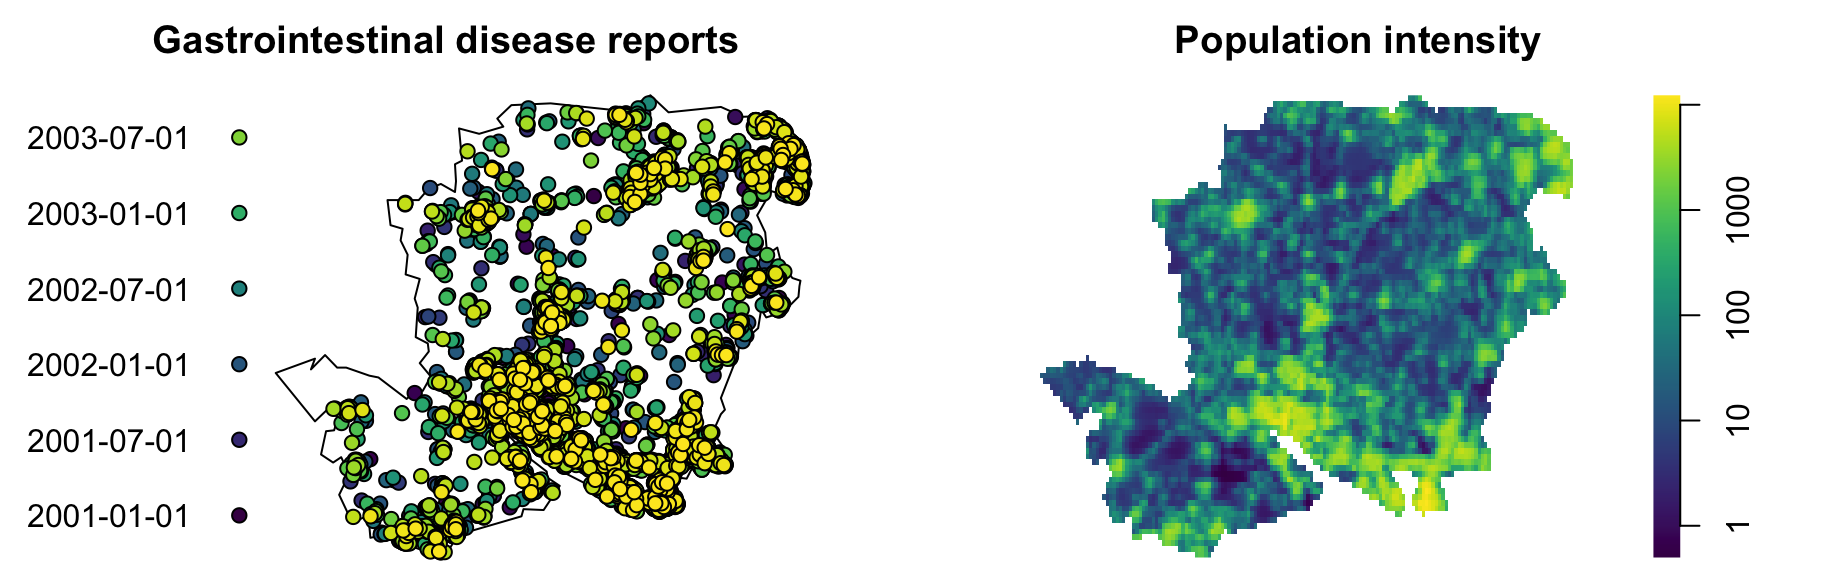
\includegraphics[width=\textwidth]{stpointprocess_files/figure-latex/stpointpattern-1} 

}

\caption{Left: Locations of 10443 reports of non-specific gastrointestinal disease in Hampshire from January 2001 to July 2003. The time is treated as a quantitative mark where darker dots correspond to the older events, and lighter dots match the most recent reports. Right: Hampshire population density averaged over the years 2001-2003. The colour map is evenly-spaced on a logarithmic scale.}\label{fig:stpointpattern}
\end{figure}

\hypertarget{spatial-analysis}{%
\section{Spatial analysis}\label{spatial-analysis}}

\hypertarget{sectionintensity}{%
\subsection{Spatial intensity and relative risk}\label{sectionintensity}}

The \emph{first-order intensity function} or the \emph{intensity} of a point process can be defined as the expected number of events per unit space, or mathematically (P. J. Diggle 2013),
\[
\lambda(\mathbf{u})=\lim_{|\text{d}\mathbf{u}|\rightarrow 0}\frac{\mathbb{E}N(\text{d}\mathbf{u})}{|\text{d}\mathbf{u}|},
\]
where \(N()\) denotes the number of points of a region. In the inhomogeneous case, we can compute a kernel smoothed intensity function from a point pattern \(\{\mathbf{u}_i\}_{i=1}^n\) without the temporal coordinates. The estimator is given by
\begin{equation}
    \hat{\lambda}(\mathbf{u})=\frac{1}{e^2(\mathbf{u})}\sum_{i=1}^{n}\kappa_{\epsilon}^{2}(\mathbf{u}-\mathbf{u}_i), \quad \text{and} \quad e^2(\mathbf{u})=\int_{W} \kappa_{\epsilon}^{2}(\mathbf{s}-\mathbf{u}) \text{d} \mathbf{s},
    \label{eq:lambdaspatial}
\end{equation}
where \(\mathbf{u}\in W\) and \(\kappa_{\epsilon}^{2}\) is a two-dimensional Gaussian kernel. \(e()\) is known as \emph{uniform edge correction} and is intended to correct the bias of the estimation at the edges of the region (Adrian Baddeley, Rubak, and Turner 2015). One of the most challenging considerations is selecting the bandwidth \(\epsilon\); there is no single best procedure for doing that, but the estimation can be improved by using a spatially varying bandwidth despite its computational complexity (Tilman M. Davies and Baddeley 2018). For computing the adaptive estimate of the intensity function, we use the \texttt{adaptative.density()} function of the \pkg{spatstat.explore} package,

\begin{verbatim}
# This takes roughly 12 seconds to be executed in an
# iMAC 2019, 3GHz intel core i5 processor with 16GB of RAM (hereinafter)
SpatialDens <- adaptive.density(X, method = "kernel", edge = T)
\end{verbatim}

The estimated intensity is shown in Figure \ref{fig:adaptativeintensities} (left). We can see a high concentration of cases (more than two per square kilometre) in Southampton and its coastal environs. More to the north, there are also local foci in Winchester (the centre of the study region) and the primary urban centres located in the north and northeast of the study region.

The \emph{kernel log relative risk} or \emph{density ratio function} is a descriptor aimed to compare two estimated densities on the study region \(W\). In epidemiology, it is handy to examine disease risk fluctuations based on case and control samples. In recent years, many improvements have been developed to the estimation methodology, including spatially adaptive smoothers and inference based on asymptotic theory (T. M. Davies, Marshall, and Hazelton 2018). The related techniques are implemented in the \pkg{sparr} package. Given two spatial point patterns, \(X\), with intensity \(\hat{\lambda}(\mathbf{u}|X)\) (that can be thought of as cases) and \(Y\), with intensity \(\hat{\lambda}(\mathbf{u}|Y)\) (that can be thought of as controls); the estimated log relative risk is defined as
\begin{equation}
    \hat{r}(\mathbf{u})=\log \left\{\frac{\hat{\lambda}(\mathbf{u}|X)}{\hat{\lambda}(\mathbf{u}|Y) } \cdot \frac{n_Y}{n_X} \right\}, \quad \mathbf{u} \in W,
    \label{eq:relrisk}
\end{equation}
where \(n_X\) and \(n_Y\) are the number of points of \(X\) and \(Y\), respectively. When \(\hat{r}(\mathbf{u}) \approx 0\), the densities are roughly the same; peaks greater than zero mean a higher local ratio of cases to controls, and \(\hat{r}(\mathbf{u}) < 0\) indicates lack of concentration of cases than controls.

Here, we compute the relative risk by comparing the point pattern of gastrointestinal infections and a point pattern with controls derived from a random sample of the underlying population. We first generate a set of random controls by simulating \(n=1443\) locations with intensity proportional to the population density using the \texttt{rpoispp()} function of package \pkg{spatstat.random}. In order to do that, we calculate the population density as the population intensity normalised by its mass (its integral over the observation window) calculated by using the function \texttt{integral.im()} of the package \pkg{spatstat.geom} in each region of Hampshire. Then we can evaluate expressions involving one or more pixel images through the \texttt{eval.im()} function of package \pkg{spatstat.geom},

\begin{verbatim}
N <- integral.im(PopDens) 
n <- X$n
ControlDens <- eval.im((PopDens / N) * n)
Controls <- rpoispp(ControlDens)
\end{verbatim}

Then we assign Hampshire's window to the new point pattern by using the \texttt{Window()} function of package \pkg{spatstat.geom},

\begin{verbatim}
Window(Controls) <- X$window
\end{verbatim}

For estimating the relative risk, we use the \pkg{sparr} package to perform an adaptive smoothing adequately designed to deal with the reduced smoothing in densely populated areas. The code

\begin{verbatim}
# This takes roughly 22 seconds to be executed 
library(sparr)
RelativeRisk <- risk(f = X, g = Controls, adapt = T, 
                     pilot.symmetry = "pooled", tolerate = T)
\end{verbatim}

takes both point patterns (cases \texttt{f} and controls \texttt{g}), computes an adaptive smoothing for estimating the risk, and computes asymptotic tolerance contours as per Hazelton and Davies (2009). Maps displayed in Figure \ref{fig:adaptativeintensities} showing the intensity and relative risk estimates are produced by executing

\begin{verbatim}
par(mfrow = c(1, 2), mar = c(0,0,2,0.5)) 
plot(SpatialDens, col = viridis(1200), auto.axes = F,
     main = "Adaptative kernel intensity estimate", box = F)
plot(RelativeRisk, auto.axes = F, tol.type = "upper", 
     main = "Relative risk estimate")
\end{verbatim}

\begin{figure}

{\centering 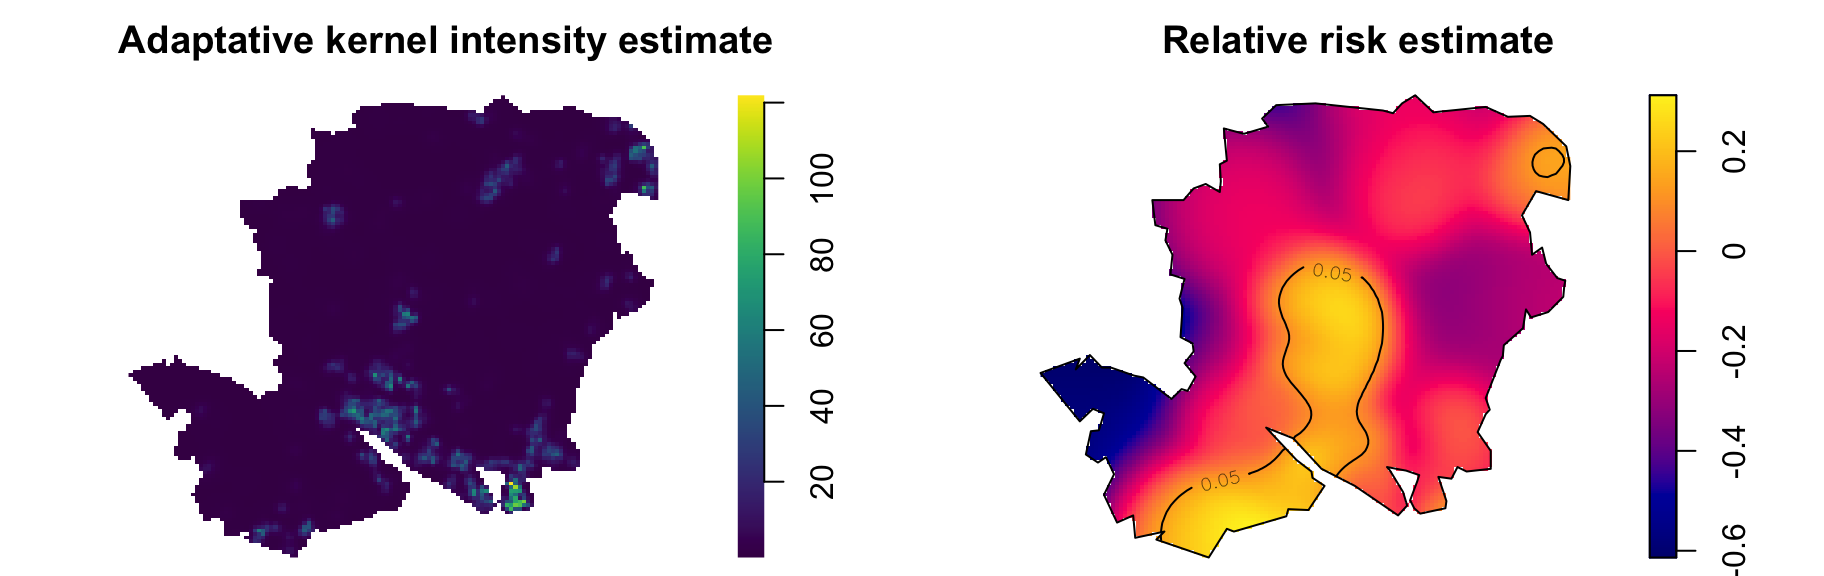
\includegraphics[width=\textwidth]{stpointprocess_files/figure-latex/adaptativeintensities-1} 

}

\caption{Left: Adaptive bandwidth kernel estimate of intensity for the gastrointestinal data. The intensity is expressed as number of reports per squared kilometre. Right: Adaptive spatial log-relative risk of non-specific gastrointestinal disease, with asymptotic tolerance contours for elevated risk.}\label{fig:adaptativeintensities}
\end{figure}

Figure \ref{fig:adaptativeintensities} (right) provides pointwise areas of significant high relative risk. The null hypothesis is \(H_0: r(\mathbf{u})=0\), against an alternative of increased local risk \(H_1:r(\mathbf{u})>0\) for a point \(\mathbf{u}\in W\). We superimpose the contours corresponding to significant values on the log relative risk surface. They are known as tolerance contours and allow us to identify areas of high risk (Kelsall and Diggle 1995). The relative abundance of gastrointestinal disease reports appears to be significantly higher in some areas where the intensity is not necessarily higher. Nor does the relative risk appear to increase in Southampton (located on the southern coast), the region's most urbanised area.

\hypertarget{second-order-descriptors}{%
\subsection{Second-order descriptors}\label{second-order-descriptors}}

\hypertarget{pair-correlation-and-k-functions}{%
\subsubsection{\texorpdfstring{Pair correlation and \(K\)-functions}{Pair correlation and K-functions}}\label{pair-correlation-and-k-functions}}

The \emph{second-order intensity function} \((\lambda^{(2)}(\mathbf{u}_1,\mathbf{u}_2), \mathbf{u}_1,\mathbf{u}_2\in W)\) is, in point processes, analogous to the covariance function in classical statistics (Adrian Baddeley, Rubak, and Turner 2015). Also known as \emph{product density function,} the second-order intensity function represents the infinitesimal two-dimensional joint distribution of the points. A more friendly summary statistic is the \emph{pair correlation function}, which is the standardised probability density that an event occurs in each of two small spatial volumes \(\text{d} \mathbf{u}_1\) and \(\text{d} \mathbf{u}_2\). For CSR (Complete Spatial Random) point processes, the covariance is zero, and the pair correlation function takes the value of one (P. J. Diggle 2013). Different values than these benchmarks indicate how likely a pair of events will occur at the specified locations than in a CSR process with the same intensity; i.e., larger values indicate clustering, and smaller values indicate regularity. The pair correlation is defined as
\begin{equation}
    g(\mathbf{u}_1,\mathbf{u}_2)=\frac{\lambda^{(2)}(\mathbf{u}_1,\mathbf{u}_2)}{\lambda(\mathbf{u}_1)\lambda(\mathbf{u}_2)}, \qquad \mathbf{u}_1,\mathbf{u}_2\in W.
    \label{eq:spatialpcf}
\end{equation}
Whenever the intensity function of a point process is bounded away from zero and its pair correlation function depends only on the difference vector \(r =||\mathbf{u}_1 - \mathbf{u}_2||\), the point process is called \emph{second-order intensity reweighted stationary} (SOIRS) and \emph{isotropic}. For estimating the pair correlation function, consider a point pattern \(X=\{\mathbf{u}_{i}\}_{i=1}^n\) with \(n\) points, then
\begin{equation}
    \hat{g}(r)=\frac{1}{2\pi} \sum_{i=1}^n \sum_{j\neq i}
    \frac{\kappa_{\epsilon}(||\mathbf{u}_{i}-\mathbf{u}_{j}||- r)}{\hat{\lambda} ( \mathbf{u}_{i}) \hat{\lambda} (\mathbf{u}_{j}) ||\mathbf{u}_{i}-\mathbf{u}_{j}|| w_{ij}}.
    \label{eq:gestimada1}
\end{equation}
Several parameters must be set before the estimation: a suitable interval for the spatial distances \(r\), a bandwidth \(\epsilon\), a one-dimensional kernel \(\kappa_{\epsilon}(\cdot)\) (Epanechnikov's kernel is usually recommended), a type of divisor (factor \(||\mathbf{u}_{i}-\mathbf{u}_{j}||\) in the denominator of Eq. \eqref{eq:gestimada1} can be replaced by \(r\), this option brings a pole, i.e., an indetermination, in \(r=0\) (Wong and Stoyan 2021)); and an edge correction \(w_{ij}\) correcting for the loss of information of outsider points close to the edges. \pkg{spatstat} usually has smart defaults for these parameters based on the knowledge of the descriptors, which many authors have contributed. For this part, we use a fixed-bandwidth kernel estimate, with bandwidth set by Scott's rule of thumb (Scott 2015), through the function \texttt{bw.scott()} of the package \pkg{spatstat.explore}, as we need simulations where the intensity has to be estimated time after time. We employ the function \texttt{density.ppp()} of package \pkg{spatstat.explore} that provides a fixed bandwidth kernel smoothed intensity function from a point pattern according to Eq. \eqref{eq:lambdaspatial}.

\begin{verbatim}
sigmaD <- bw.scott(X)
MD <- density.ppp(X, diggle = T, positive = T, sigma = sigmaD)
MP <- density.ppp(X, diggle = T, sigma = sigmaD, at = "points")
\end{verbatim}

In the above implementation, \texttt{diggle\ =\ T} sets the Jones-Diggle edge correction (P. J. Diggle 1985), \texttt{at\ =\ \textquotesingle{}points\textquotesingle{}} means that the intensity is computed only at the points of \(X\), and \texttt{sigma} is the bandwidth, which in this case is \(3.5\)km for the horizontal axis and \(4.19\)km for the vertical axis. In the case of the bandwidth for the pair correlation function, we employ a composite likelihood approach (Jalilian and Waagepetersen 2018) by using the function \texttt{bw.pcf()} of library \pkg{spatstat.explore} with the parameter \texttt{cv.method\ =\ \textquotesingle{}compLik\textquotesingle{}}; the parameter \texttt{divisor\ =\ \textquotesingle{}d\textquotesingle{}} refers to the term \(||\mathbf{u}_{i}-\mathbf{u}_{j}||\) in Eq. \eqref{eq:gestimada1}, which can be replaced by \(r\) (Jalilian and Waagepetersen 2018), and \texttt{lambda} is the estimate of the intensity. We then write

\begin{verbatim}
# Time consuming: This takes roughly 24 minutes to be executed 
bwG <- bw.pcf(X, cv.method = "compLik", divisor = "d", lambda = MP)
\end{verbatim}

and obtain a bandwidth value of \(2.7\)km. Note that this function can warn of undetermined contributions to the pair correlation. These caveats come from the divisor, which, when too small, can conflict with the numerical tolerance of R and eventually lead to indeterminacy. The \pkg{spatstat} package fixes this by simply removing the problematic values.

Before going further with the estimation of the pair correlation function, let us take a look into another classical second-order descriptor, the \emph{inhomogeneous \(K\)-function}, which in the SOIRS case, can be defined as
\[
    K(r)=2\pi \int_0^r sg(s)\text{d} s.
\]
For spatial Poisson point processes \(K(r)=\pi r^2\). \pkg{spatstat} chooses a suitable range for \(r\) values based on some rules of thumb depending on geometric attributes of the process or the average intensity in the region. We decide to choose a proportion of 70\% of the maximum value for \(r\) proposed by \pkg{spatstat.explore} through the \texttt{rmax.rule()} function, and set of 70 (71 including zero) different values for \(r\),

\begin{verbatim}
r0 <- 0.7 * rmax.rule("K", X$window, intensity(X))
rr <- seq(0, r0, length.out = 71)
\end{verbatim}

The classical estimator of the spatial \(K\)-function is given by
\begin{equation*}
    \hat{K}(r)= \sum_{i=1}^n \sum_{j \neq i}
    \frac{\mathbf{1}\left[|| \mathbf{u}_{i}-\mathbf{u}_{j} || \leq r\right]}{\hat{\lambda}(\mathbf{u}_{i}) \hat{\lambda} (\mathbf{u}_{j}) w_{ij}}.
    \label{eq:Kstimatormoller}
\end{equation*}
Where \(\mathbf{1}[\cdot]\) is the indicator function. An alternative descriptor defined as \(L(r)-r= \sqrt{K(r) / \pi}-r\), and its straightforward estimator \(\hat{L}(r)-r\) are intended for stabilising the variance (Besag 1977).

In addition to the estimation of the second-order descriptors, their standard deviation and confidence intervals are desirable for the analysis; this is not always simple, not even in the Poisson case, as there is dependence between the contributions of different points to the descriptor. However, we can use Monte Carlo simulation for computing envelopes through computational efforts. We use command \texttt{envelope()} of the \pkg{spatstat.explore} for getting the observed descriptor as well as its simulated counterparts.

We note that although Monte Carlo testing is generally used in point process contexts, it becomes invalid when the null hypothesis is composite, i.e., when parameters, such as the intensity function, must be estimated prior to the computing of the envelopes, which is our case for inference about the second-order descriptors. For dealing with such composite hypotheses, an extra set of simulations is needed to perform a balanced two-stage test (Adrian Baddeley et al. 2017). The \pkg{GET} package performs global envelope tests (where the significance level is controlled simultaneously for all the functions) for the second-order descriptors and provides a graphical interpretation (see, e.g., Myllymäki et al. 2017). We perform a global rank envelope test with the extreme rank length measure and retrieve the \(p\)-value. We warn the reader that this procedure of computing envelopes and two-stage Monte Carlo testing is computationally demanding. We calculate the first set of \(39\) envelopes for the centred \(L\)-function. This selection gives 39 (simulated) + 1 (observed) independent samples; it comes from classical settings of point process simulation (Ripley 1977; Adrian Baddeley, Rubak, and Turner 2015; Adrian Baddeley et al. 2017). We use the \texttt{envelope.ppp()} function of the \pkg{spatstat.explore} package; this function computes simulation envelopes of a summary function,

\begin{verbatim}
# Time consuming: This takes roughly 3 minutes to be executed 
L1 <- envelope(X, nsim = 39, savefuns = TRUE, fun = "Linhom", diggle = T,
               transform = expression(.-r), sigma = sigmaD, r = rr, 
               simulate = expression(rpoispp(lambda = MD)), verbose = F)
\end{verbatim}

Then we generate another set of inhomogeneous Poisson point patterns with the estimated intensity,

\begin{verbatim}
Simpatterns <- rpoispp(lambda = MD, nsim = 39)
\end{verbatim}

We design a function to calculate the intensity for each point pattern and to compute envelopes with point patterns simulated from the new intensity,

\begin{verbatim}
simL <- function(rep) {
  sim_fit <- density.ppp(Simpatterns[[rep]], diggle = T, 
                         sigma = sigmaD, positive = T)
  envelope(Simpatterns[[rep]], nsim = 39, savefuns = T, fun = "Linhom", 
           transform = expression(.-r), r = rr, diggle = T, sigma = sigmaD,
           simulate = expression(rpoispp(lambda = sim_fit)))
}
\end{verbatim}

Now we apply the function for every point pattern of the list to get a list of envelope objects. This process is very slow as 39 \(L\)-functions have to be computed for each point pattern. We employ the package \pkg{foreach} to use multiple processors to accelerate this procedure in combination with the \pkg{parallel} and \pkg{doParallel} packages. The function \texttt{detectCores()} of the package \pkg{parallel} automatically detects the computer's CPU cores and the function \texttt{registerDoParallel()} of the \pkg{doParallel} package is used to register a parallel backend in the computer. The \texttt{foreach()\ \%dopar\%} function returns a list with the result of applying a function over every element of the main argument by using the registered cores of the computer processor,

\begin{verbatim}
# Time consuming: This takes roughly 21 minutes to be executed 
library(foreach)
library(doParallel)
c0 <- parallel::makeCluster(detectCores() - 1)
doParallel::registerDoParallel(c0)
L.ls <- foreach(i = 1:39, .packages = c("spatstat")) %dopar% {simL(i)}
parallel::stopCluster(c0)
\end{verbatim}

Finally, we perform the adjusted test using the function \texttt{GET.composite()} of the \pkg{GET} package and plot the envelopes. In this case, we are interested in establishing a possible positive departure of the observed centred \(L\)-function and its simulated counterparts. Thus, we set \texttt{alternative\ =\ "greater"}, \texttt{type\ =\ \textquotesingle{}erl\textquotesingle{}}, which performs a rank envelope test based on extreme rank lengths (Myllymäki et al. 2017) based on several minimal pointwise ranks; and use the \CRANpkg{ggplot2} (Wickham 2016) package for the plots,

\begin{verbatim}
library(GET)
library(ggplot2)
resL <- GET.composite(X = L1, X.ls = L.ls, type = "erl", 
                      alternative = "greater", savefuns = T)
\end{verbatim}

\begin{figure}

{\centering 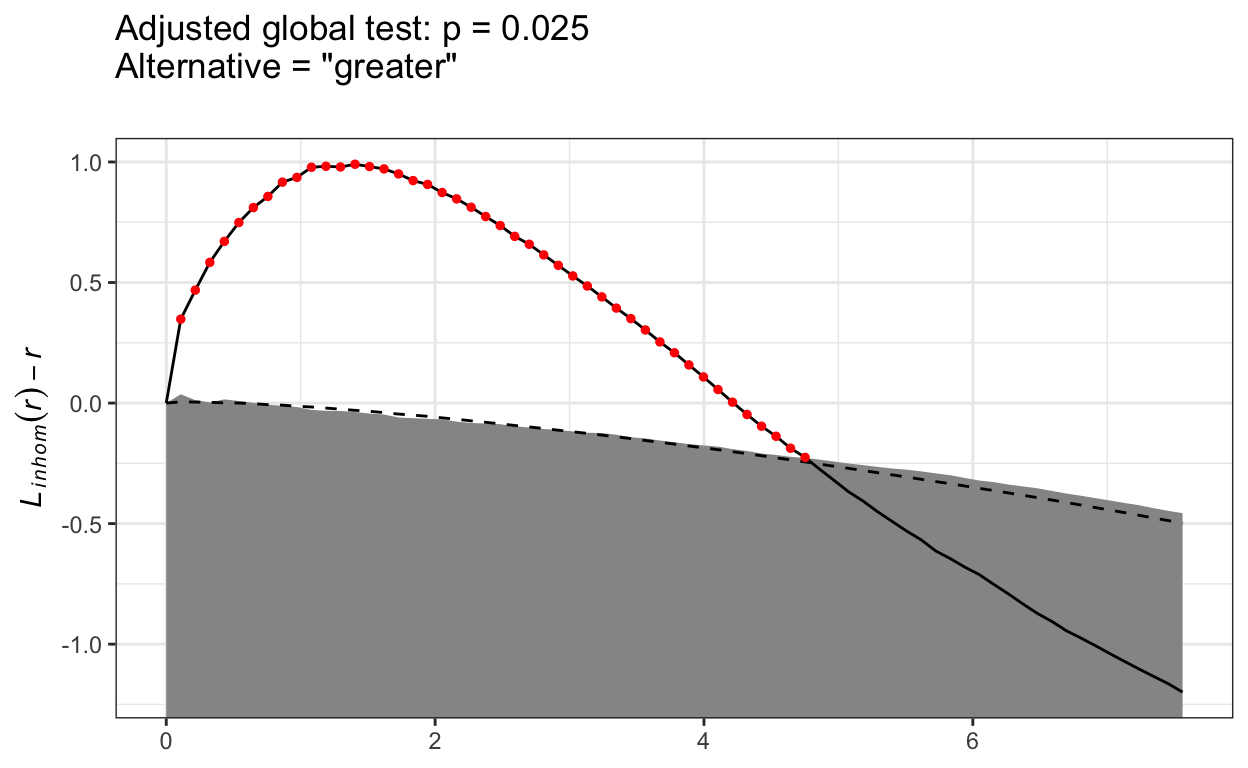
\includegraphics[width=0.75\linewidth]{stpointprocess_files/figure-latex/kandgspatial-1} 

}

\caption{Graphical clustering tests of Hampshire data based on the $L$-functions. The gray bands represent the $95\%$ global envelope. Red dots stand for the second-order descriptors outside the envelopes.}\label{fig:kandgspatial}
\end{figure}

Figure \ref{fig:kandgspatial} shows the output of the rank envelope test. The rejection is explained by the attractive behaviour of gastrointestinal disease cases at short distances. The red-dot line indicates this clustering behaviour up to 5km, which shows a departure from the narrow grey band that represents the 95\% adjusted rank envelope, i.e., the rank envelope that considers the composite hypothesis. Note that the more simulations, the better results for the test (Myllymäki et al. 2017). The dashed black line represents the central function (the mean) of only the first set of simulations; note that this function is not the mean value of the grey ribbon as it comes from envelopes under the composite null hypothesis. We find a significant positive departure from the envelopes up to approximately \(5\)km; this means that observed data are more clustered in distances below \(5\)km than might be expected in Poisson point patterns with the same intensity, and this clustering is statistically significant.

\hypertarget{spatio-temporal-analysis}{%
\section{Spatio-temporal analysis}\label{spatio-temporal-analysis}}

\hypertarget{spatio-temporal-intensity-and-relative-risk}{%
\subsection{Spatio-temporal intensity and relative risk}\label{spatio-temporal-intensity-and-relative-risk}}

\hypertarget{first-order-separability}{%
\subsubsection{First-order separability}\label{first-order-separability}}

Spatio-temporal point processes analyses can be carried out when every data point has associated geographic and time information. In these cases, estimating the first-order intensity function constitutes a primary interest. The intensity function provides information about the joint distribution of the spatial and temporal locations. Usually, this distribution is simplified by assuming, for example, separability. A point process is referred to as \textit{separable} when its spatio-temporal intensity function can be factorised as
\[
    \lambda(\mathbf{u},v) = \lambda_1(\mathbf{u}) \lambda_2(v), \quad  \mathbf{u} \in W,v \in T,
\]
where \(\lambda_1(\cdot)\) and \(\lambda_2(\cdot)\) are non-negative functions of space and time, respectively. Authors often take separability for granted as it is a very pragmatic working assumption, but it should be tested before choosing an estimator. There are some specialised separability tests available in the literature. We use the package \CRANpkg{kernstadapt} (González and Moraga 2022b) to test separability in our example by considering a division of the temporal interval \(T=[1,1095]\) into 16 disjoint equally-spaced sub-intervals. We split the spatial window \(W\) into 20 disjoint rectangular subsets with roughly the same area. As the separability of the intensity might be thought of as the independence of two random variables, it can be tested by a simple \(\chi^2\)-test as proposed by Ghorbani et al. (2021), where the null hypothesis is separability. The test bases on the counts of points in disjoint spatial and temporal sub-regions; when there are expected counts of individual cells below 5, the authors recommend a Fisher's test. We employ Fisher's test calculating the \(p\)-value by Monte Carlo simulation (5000 replicates):

\begin{verbatim}
# This takes roughly 20 seconds to be executed 
SepTest <- separability.test(Aegiss, nx = 5, ny = 4, nt = 16, nperm = 50000)
\end{verbatim}

\begin{verbatim}
SepTest
\end{verbatim}

\begin{verbatim}
#> 
#>  Separability test based on Fisher's for counting data
#> 
#> data:  Point pattern Aegiss
#> p-value = 0.00346
#> alternative hypothesis: The point pattern Aegiss is not spatio-temporal separable
\end{verbatim}

As the \(p\)-value is significant, we opt for estimating the spatio-temporal intensity in a non-separable fashion. We estimate the intensity by employing the following estimator, which uses a Gaussian kernel for all coordinates (Choi and Hall 1999; González, Hahn, and Mateu 2019; Ghorbani et al. 2021)
\begin{equation}
    \hat{\lambda}(\mathbf{u},v)=\sum_{i=1}^{n}\frac{\kappa_{\epsilon}^{2}(\mathbf{u}-\mathbf{u}_i)\kappa_{\delta}^{1}(v-v_i)}{e^2(\mathbf{u}_i)e^1(v_i)},
    \label{eq:lambdaNS}
\end{equation}
where
\[
e^2(\mathbf{u}_i)=\int_{W} \kappa_{\epsilon}^{2}(\mathbf{u}_i-\mathbf{s})\text{d} \mathbf{s}, \quad \text{and}\quad e^1(v_i)=\int_{T} \kappa_{\delta}^{1}(v_i-w)\text{d} w;
\]
and where \(\kappa_{\epsilon}^{2}\) and \(\kappa_{\delta}^{1}\) are the two- and one-dimensional Gaussian kernels with bandwidths \(\epsilon\) and \(\delta\).

In this case, we use a fixed spatial bandwidth calculated by a rule of thumb that depends on the short size of the window and a temporal one calculated through the function \texttt{bw.nrd()}. Notice that the spatio-temporal estimator given in Eq.\eqref{eq:lambdaNS} resembles the spatial one given in Eq.\eqref{eq:lambdaspatial}, with an extra kernel weight for the temporal component. On the other hand, as the spatial edge correction, due to P. J. Diggle (1985), is already implemented in the function \texttt{density.ppp()} of \pkg{spatstat.explore}, we must calculate the temporal one. We employ the generic function \texttt{bw.nrd0()} of package \pkg{stats} for the temporal bandwidth, which uses Silverman's rule-of-thumb (Silverman 1986) for choosing the bandwidth of a Gaussian kernel density estimator. For computing the edge correction, we take advantage of the properties of the normal distribution noticing that \(e^1(v_i)=\mathbb{P}(Y_i \in T)\) where \(Y_i \sim N(v_i, \delta^2)\), indeed,

\begin{verbatim}
Times <- Aegiss$marks
bwt <- bw.nrd0(Times)
edgewt.t <- pnorm((max(Times) - Times) / bwt) - pnorm((min(Times)- Times) / bwt) 
\end{verbatim}

Then we proceed to calculate the non-separable estimator. To quicken the computation, for each fixed time \(t_0\), we take temporal bins \(t\in [t_0-3\delta, t_0+3\delta]\), as the normal distribution practically vanishes at larger or smaller values, then we compute the temporal kernel values and attach them to the spatial kernel as weights,

\begin{verbatim}
# This takes roughly 44 seconds to be executed 
nonseparable <- function(time){
    contrib <- (Times >= time - 3 * bwt) & (Times <= time + 3 * bwt)
    Wh <- dnorm(x = Times[contrib], mean = time, sd = bwt) / edgewt.t[contrib]
    density.ppp(X[contrib], weights = Wh, diggle = TRUE)
}
nonsep <- lapply(unique(Times), nonseparable)
\end{verbatim}

We have 1047 intensity estimates corresponding to each of the 1047 different times; note that 1047 is the size of the temporal coordinates set and not the maximum temporal value (1095). We decide to plot a subset of them, namely the estimates corresponding to times \(01/01/2001\), \(01/01/2002\), \(01/01/2003\) and \(12/31/2003\).

\begin{verbatim}
n.slices <- which(unique(timelabels) %in% as.Date(c("2001-01-01", "2002-01-01", 
                                                    "2003-01-01", "2003-12-31")))
Snap <- list(nonsep[[n.slices[1]]], nonsep[[n.slices[2]]], 
             nonsep[[n.slices[3]]], nonsep[[n.slices[4]]])
plot.imlist(Snap, equal.ribbon = T, ncols = 4, box = F, main = "", log = F,
            main.panel = unique(timelabels)[n.slices], col = viridis(1200),
            ribscale = 100,  mar.panel=c(0, 0, 1, 1), panel.end = X$window)
\end{verbatim}

\begin{figure}

{\centering 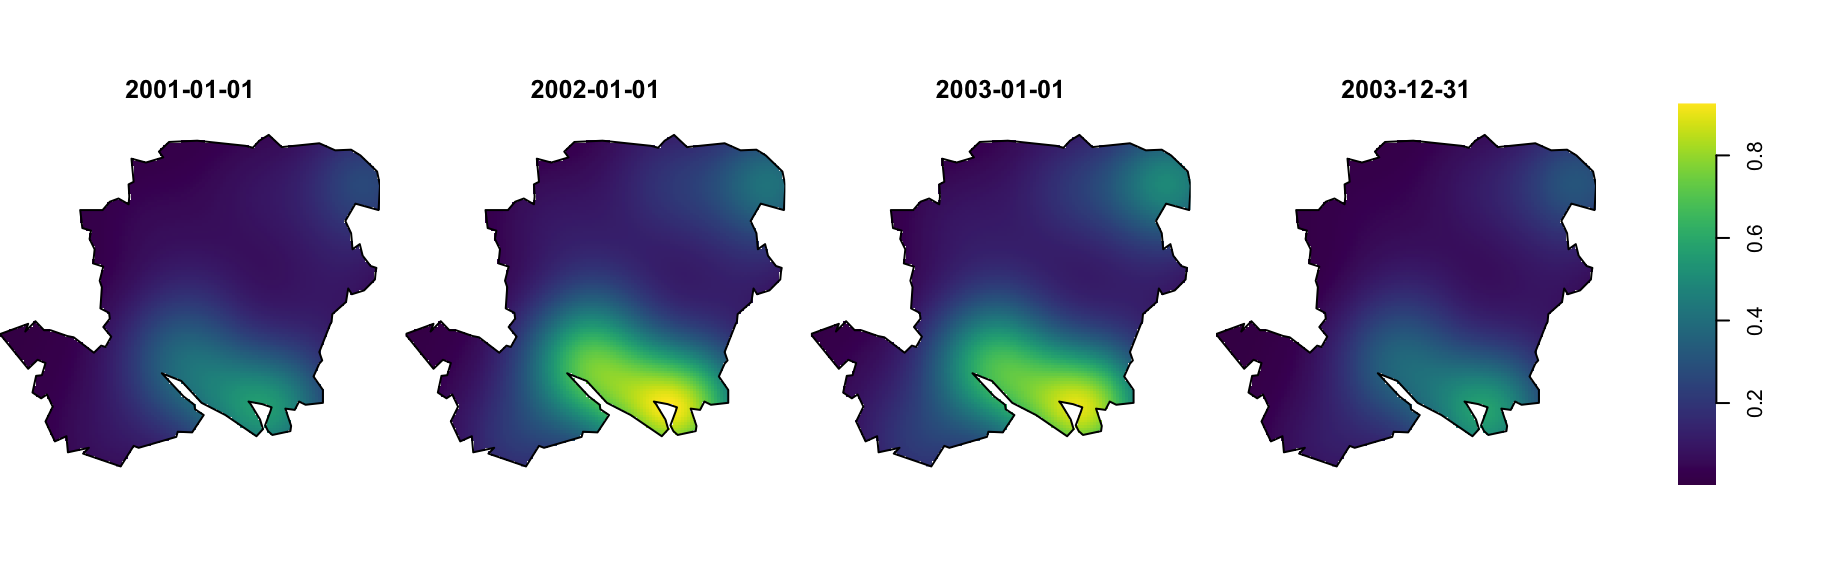
\includegraphics[width=1\linewidth]{stpointprocess_files/figure-latex/snapshotsintensity-1} 

}

\caption{Temporal snapshots of the intensity $\hat{\lambda}(\mathbf{u},v)$, of non-specific gastrointestinal reports in Hampshire, estimated in a non-separable way through Gaussian kernels. The units are rescaled by $100$.}\label{fig:snapshotsintensity}
\end{figure}

In the spatio-temporal case (Figure \ref{fig:snapshotsintensity}), we can see a behaviour in the intensity of cases much lower than in the spatial case (Figure \ref{fig:adaptativeintensities} (left)) due to the temporal granularity. This scale difference is due to the number of events per unit of time, which is not considered in the only spatial estimation. When considering the temporal dimension, the total points must be divided by the number of bins in the temporal grid where the estimation is made. Therefore, there are fewer points per unit area at each time than only when spatial coordinates are considered.

The intensity maintains some urban centres as foci over time, especially those in the south, for example, in Portsmouth, where there is a high concentration of cases between 2002 and 2003.

In the next section, we show how to compute spatio-temporal descriptors. To do that, we need to know the intensity values at every point of the point pattern. We can extract the intensity values by using the \texttt{safelookup()} of \pkg{spatstat.geom}. Then, we attach those values, and the dates, as a mark to each point by using the operator \texttt{\%mark\%},

\begin{verbatim}
lambda <- NULL
for (i in 1:length(nonsep)) {
    lambda <- c(lambda, safelookup(nonsep[[i]], 
    Aegiss[marks(Aegiss) == unique(Times)[i]]))
}
PP <- X %mark% data.frame(time = Aegiss$marks, Lambda = lambda)
\end{verbatim}

\hypertarget{spatio-temporal-relative-risk}{%
\subsubsection{Spatio-temporal relative risk}\label{spatio-temporal-relative-risk}}

The concept of relative risk straightforwardly extends to the spatio-temporal domain. In this regard, we must make additional considerations; for example, the spatial relative risk can be conditioned to a specific time (T. M. Davies, Marshall, and Hazelton 2018). Analogous to the classic probability, in the spatio-temporal context, the idea of conditioning on a specific time \(v=t_0\) comes naturally. This means that for a fixed instant \(t_0\), we consider the spatial density function given that time. Mathematically, it is calculated by normalising the spatio-temporal density by the density of the temporal coordinates evaluated at the fixed time \(t_0\). On the other hand, if it is not conditioned to a particular time, the risk function is a function of three variables (two spatial coordinates and one temporal), which can be drawn through snapshots. Thus, we have two possible risk functions, \(r(\mathbf{u},v)\) (if plotted at a fixed time, it represents an unnormalised slice of the three-dimensional function) and \(r(\mathbf{u}|v=t_0)\) (a spatial-only snapshot of relative risk).

Given that we have population information for 2001, 2002 and 2003, we generate controls from these three population densities considering uniform times within each year. Then, we superimpose the three control point patterns into one using the \texttt{superimpose()} function of the \pkg{spatstat.geom} package. We obtain a spatio-temporal point pattern of controls that will serve as input to calculate the denominator of the relative risk.

\begin{verbatim}
Ni <- lapply(Population, integral.im)
ni <- lapply(split(Aegiss, cut(Aegiss$marks, breaks = c(0, 365, 730, 1095))), 
             npoints)
ControlDensi <- mapply(function(D, N, n) {eval.im((D / N) * n)}, 
                       D = Population, N = Ni, n = ni, SIMPLIFY = F)
Controlsi <- mapply(function(L, Breaks){
  PP <- rpoispp(lambda = L)
  marks(PP) <- sample(x = (Breaks[1] + 1):Breaks[2], 
                      size = npoints(PP), replace = T)
  return(PP)}, 
  L = ControlDensi, Breaks = list(c(0, 365), c(365, 730), c(730, 1095)), 
  SIMPLIFY = F)

Controlsi <- superimpose(as.solist(Controlsi))
Controlsi <- unmark(Controlsi) %mark% Controlsi$marks$origMarks
Window(Controlsi) <- Window(Aegiss)
\end{verbatim}

For the spatio-temporal risk estimation exercise, we return to the \pkg{sparr} package. We follow the recommendations of (T. M. Davies, Marshall, and Hazelton 2018) and set \emph{oversmoothing bandwidths} (a rule based on an optimal bandwidth upper bound for the asymptotic mean integrated squared error of the density estimate, this may be done using the command \texttt{OS.spattemp()}). The spatio-temporal densities can analysed through the command \texttt{spattemp.density()} of the \pkg{sparr} package.

\begin{verbatim}
# This takes roughly 4.87 minutes to be executed
Br <- OS.spattemp(Aegiss)
f.num <- spattemp.density(Aegiss, h = Br[1], lambda = Br[2])
d.den <- spattemp.density(Controlsi, h = Br[1], lambda = Br[2])
\end{verbatim}

In this case, interest may rise about the anomalous regions of spatio-temporal risk considering joint and conditional risks (given a time \(t\)); i.e., we are interested in testing the null hypotheses \(H_0:r(\mathbf{u},v)=0\) or \(H_0:r(\mathbf{u},|v=t)=0\) against the alternatives of high risks. We employ the \texttt{spattemp.risk()} function of \pkg{sparr} to obtain a spatiotemporal relative risk surface based on the ratio of the two kernel estimates. In addition, since doing Monte Carlo simulations to obtain \(p\)-values is very complicated from the computational point of view, asymptotic approximations are implemented in \pkg{sparr} by setting \texttt{tolerate\ =\ T},

\begin{verbatim}
# This takes roughly 5.47 minutes to be executed
st.risk <- spattemp.risk(f = f.num, g = d.den, tolerate = T)
\end{verbatim}

We proceed to extract the unconditional and conditional risk slices,

\begin{verbatim}
risk.slices <- spattemp.slice(st.risk, tt = n.slices)
\end{verbatim}

The variable \texttt{risk.slices} contains a list of lists of images, each of which corresponds to the requested times in n.slices and has the unconditional and conditional risk estimates and the \(p\)-values surfaces. We can plot the image estimates as follows:

\begin{verbatim}
plot.imlist(c(risk.slices$rr, risk.slices$rr.cond), equal.ribbon = T, ncols = 4, 
            box = F, main = "", main.panel = c(timelabels[n.slices], rep("", 4)), 
            mar.panel = c(0, 0, 1, 1), col = rocket(1200), ribmar = c(1, 3, 1, 2), 
            ribwid = 0.4, panel.end = function(i,...){
              contour(c(risk.slices$P, risk.slices$P.cond)[[i]], 
                      levels = 0.05, drawlabels = TRUE, ...)
              plot(X$window, add = T)})
\end{verbatim}

\begin{figure}

{\centering 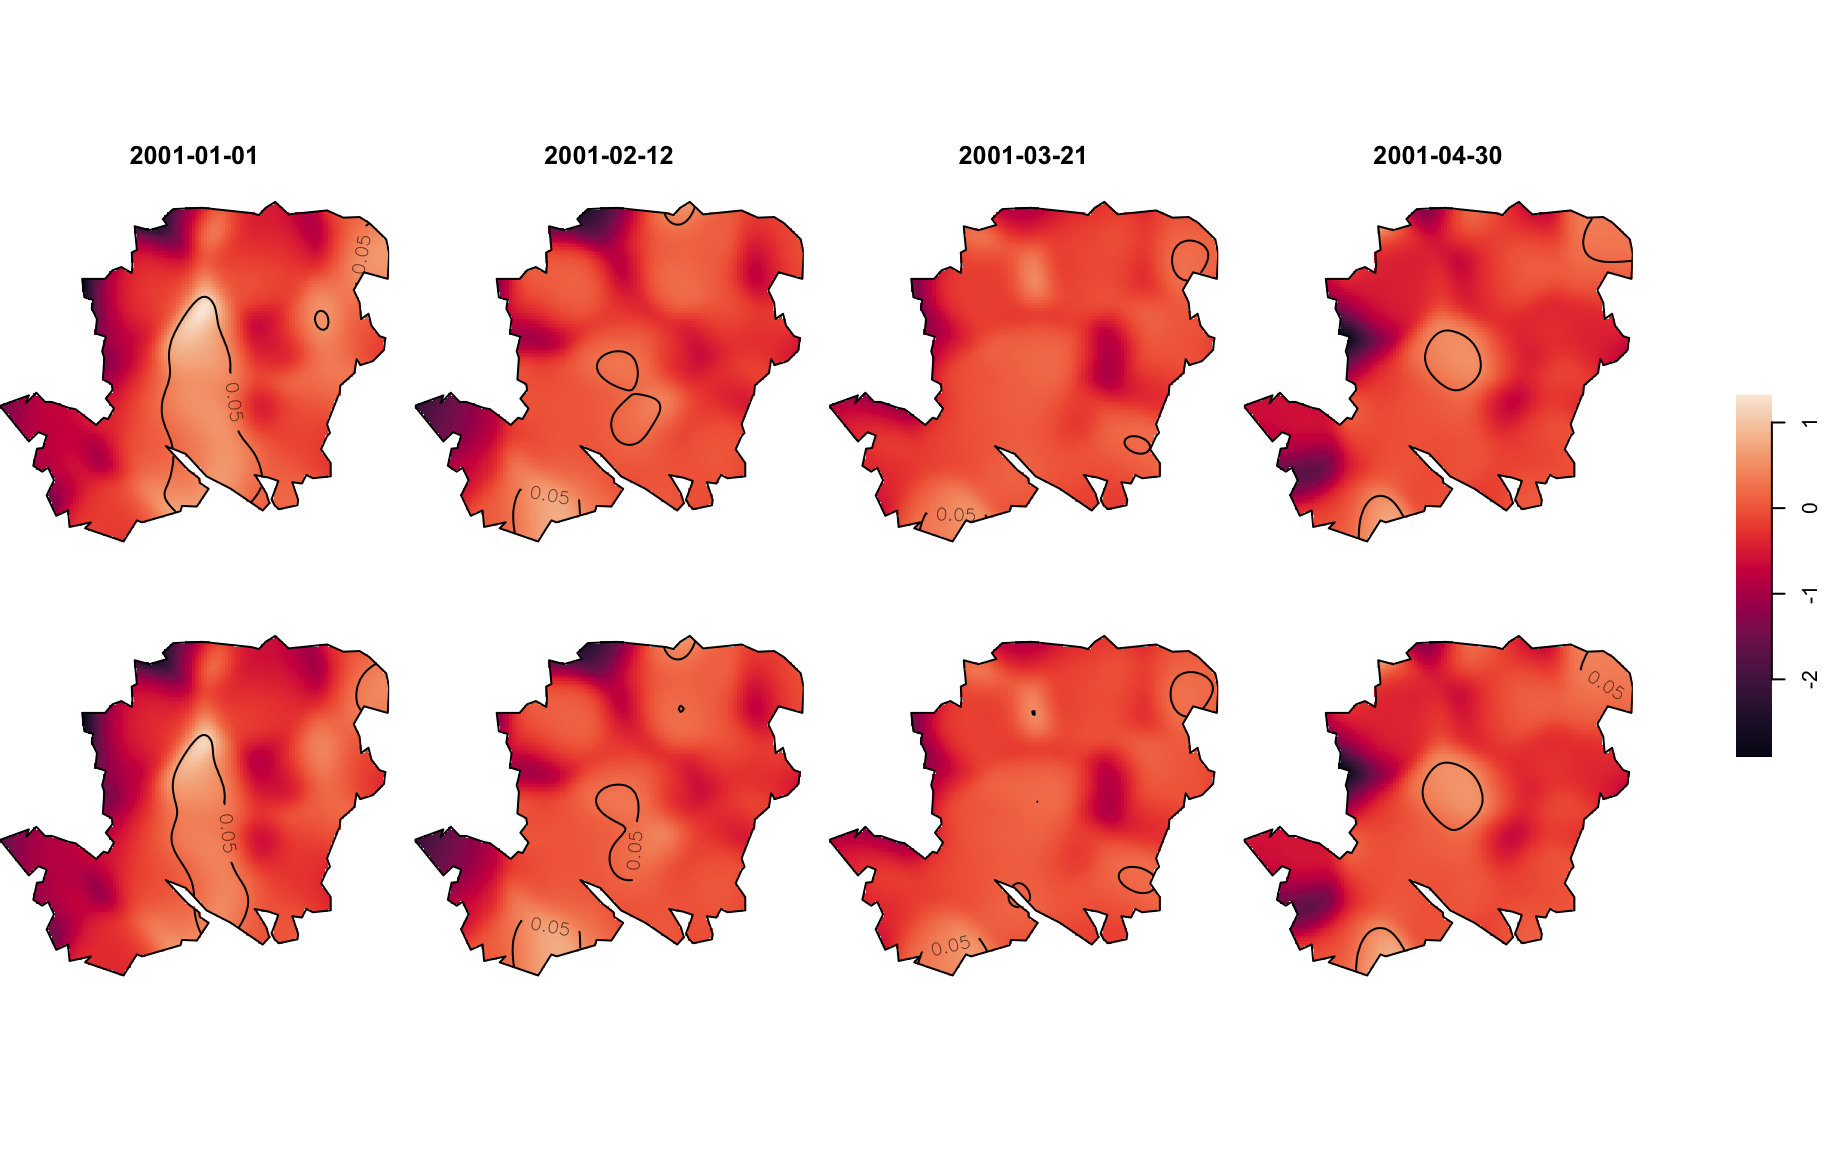
\includegraphics[width=1\linewidth]{stpointprocess_files/figure-latex/strisk-1} 

}

\caption{Temporal snapshots of the unconditional risk $\hat{r}(\mathbf{u},v)$ (top) and conditional risk $\hat{r}(\mathbf{u}|v= t)$ (where $t$ is $01/01/2001$, $01/01/2002$, $01/01/2003$ and $12/31/2003$) (bottom) of non-specific gastrointestinal disease in Hampshire. Solid lines delineate a statistical significant elevated risk at the $5\%$ level.}\label{fig:strisk}
\end{figure}

In Figure \ref{fig:strisk}, we can see how the high significant risk remains in the central Hampshire region. Although the two panels (top and bottom) look similar, there are differences. For example, in February 2001, we see how the conditional risk shows a larger statistically high area than its unconditional counterpart. We also see that the greatest risk is not present in the most densely populated areas (in this case, the south-central part of the region, where the capital is located).

\hypertarget{second-order-descriptors-1}{%
\subsection{Second-order descriptors}\label{second-order-descriptors-1}}

\hypertarget{pair-correlation-and-k-functions-1}{%
\subsubsection{\texorpdfstring{Pair correlation and \(K\)-functions}{Pair correlation and K-functions}}\label{pair-correlation-and-k-functions-1}}

Let \(\xi_1 = (\mathbf{u}_1,v_1),\xi_2 = (\mathbf{u}_2,v_2)\) be two points of \(W\times T\). The second-order intensity function \((\lambda^{(2)}(\xi_1,\xi_2), \xi_1,\xi_2\in W\times T)\) and the pair correlation function are defined in the spatio-temporal context, in the very same way as the spatial ones. For CSTR point processes, the pair correlation function takes the value of one. Values other than these benchmarks indicate how likely a pair of ``extra'' points will appear in a CSTR process with the same intensity at the specified locations; i.e., larger values indicate clustering, and smaller values indicate regularity. The pair correlation (Gabriel and Diggle 2009; Møller 2012; González et al. 2016) is defined as
\begin{equation}
    g(\xi_1,\xi_2)=\frac{\lambda^{(2)}(\xi_1,\xi_2)}{\lambda(\xi_1)\lambda(\xi_2)}, \qquad \xi_1,\xi_2\in W\times T.
    \label{eq:pcf}
\end{equation}
Second-order intensity reweighted stationarity (SOIRS) and isotropy are defined in the same vein as the spatial counterparts. For the estimation of the pair correlation function, consider a point pattern \(X=\{(\mathbf{u}_{i},v_i)\}_{i=1}^n\) with \(n\) points, the spatio-temporal pair correlation function (Eq. \eqref{eq:pcf}) may be estimated by
\[
    \hat{g}(r,t)=\frac{1}{4\pi r}
    \sum_{i=1}^n \sum_{j\neq i}
    \frac{\kappa_{\epsilon}(\|\mathbf{u}_{i}-\mathbf{u}_{j}\|- r)\kappa'_{\delta}(|v_{i}-v_{j}|-t)}{\hat{\lambda} \left( \mathbf{u}_{i},v_{i}\right) \hat{\lambda} \left(\mathbf{u}_{j},v_{j}\right) w_{ij}
    }, \quad r \in [\epsilon, r_0], t\in [\delta, t_0],
\]
where \(\kappa_{\epsilon}\) and \(\kappa'_{\delta}\) are one-dimensional kernel functions with spatial and temporal bandwidths \(\epsilon\) and \(\delta\), respectively; \(w_{ij}\) represent edge-correction weights (González et al. 2016). Selecting the bandwidths is often complicated because the estimation depends on those parameters, which means a wrong decision could be disastrous. As the second-order descriptors are distance-based, we can take advantage of some techniques for bandwidth selection. For example, for the temporal kernel, we use the \texttt{dpik()} function from the \CRANpkg{KernSmooth} package (González and Moraga 2022b), which uses the method proposed by (Sheather and Jones 1991) to estimate a suitable bandwidth,

\begin{verbatim}
library(KernSmooth)
dt <- dist(unique(Times))
ht <- dpik(dt, kernel = "epanech", gridsize = 50, scalest = "iqr")
ht <- 2 * ht
\end{verbatim}

Note that we set Epanechnikov's kernel as a default because the kernel selection is not as important as the bandwidth. We get a temporal bandwidth of \(13.5\) days (the output of the \texttt{dpik()} function). For the spatial bandwidth and upper bound \(r_0\), we use the same as obtained for the spatial summary functions. For the temporal upper bound \(t_0\), we set the 15\% of the maximum temporal distances,

\begin{verbatim}
t0 <- 0.15 * max(dt)
\end{verbatim}

We use the \pkg{stpp} package to estimate the descriptor. We first create data in spatio-temporal point format using the command \texttt{as.3dpoints()}; then, we create a two-column matrix to specify the polygonal region containing the points and set the spatial and temporal domains for the descriptor. Finally, we use the \texttt{PCFhat()} function to compute the estimate of the pair correlation function,

\begin{verbatim}
library(stpp)
FMD <- as.3dpoints(PP$x, PP$y, PP$marks$time)
s.region <- as.matrix(data.frame(x = PP$window$bdry[[1]]$x, 
                                 y = PP$window$bdry[[1]]$y))
hs <- bwG
u1 <- seq(hs, r0, length.out = 71)[-1]
v1 <- seq(ht, t0, length.out = 71)[-1]
\end{verbatim}

\begin{verbatim}
# Time consuming: This takes roughly 3.87 hours to be executed
g <- PCFhat(xyt = FMD, s.region = s.region, t.region = range(Times), 
            lambda = lambda, dist = u1, times = v1, ks = "epanech", 
            kt = "epanech", hs = hs, ht = ht)
\end{verbatim}

To visualise the descriptor, we use the \texttt{persp3D()} function of the \CRANpkg{plot3D} package,

\begin{verbatim}
library(plot3D)
par(mar = c(0,0,0,0))
persp3D(x = u1, y = v1, z = g$pcf, facets = NA, curtain = F, col =  viridis(200), 
    colkey = F, bty = "g", pch = 20, cex = 1.5, theta = 40, phi = 5, 
    border = NA, ticktype = "detailed", cex.axis = 0.5,  zlab = "",
    xlab = "spatial distances", ylab = "temporal distances")
\end{verbatim}

\begin{figure}

{\centering 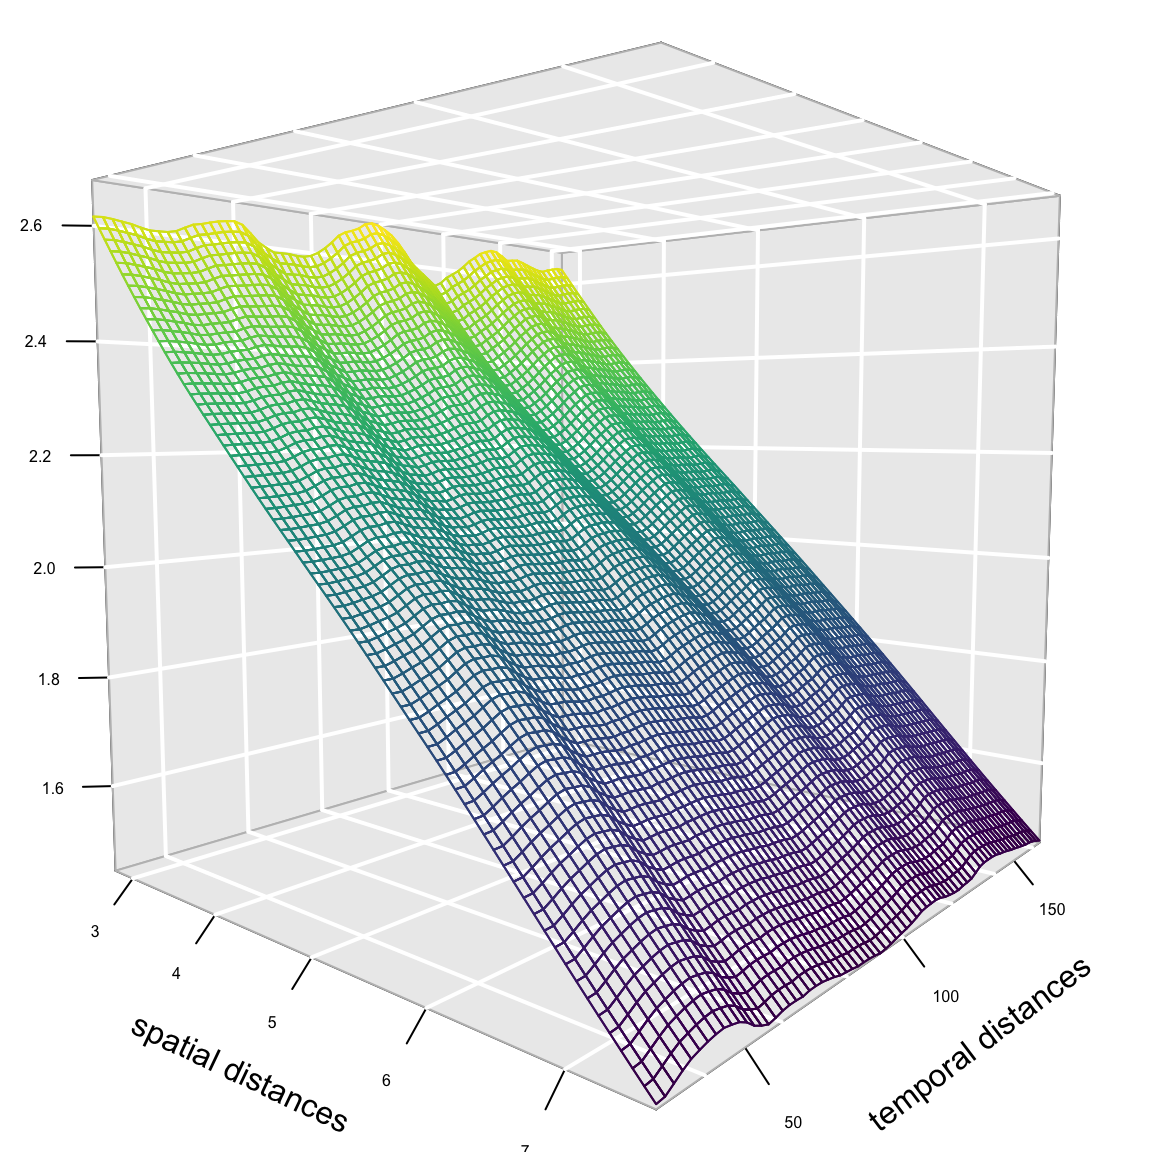
\includegraphics[width=0.65\linewidth]{stpointprocess_files/figure-latex/gfunction-1} 

}

\caption{Spatio-temporal pair correlation function estimate of non-specific gastrointestinal disease data.}\label{fig:gfunction}
\end{figure}

The \(\hat{g}(r,t)\) surface, shown in Figure \ref{fig:gfunction}, describes the spatio-temporal interaction structure of the disease; it shows clustering (\(\hat{g}(r,t)\geq 1\)) for all the distances at all times with the appearance of high clustering at small distances (up to \(5\)km) that moves towards complete spatio-temporal randomness (CSTR) for more considerable distances. We then can suspect from this behaviour that the point pattern is only clustered in the spatial dimension, i.e., the interaction between gastrointestinal reports increases as long as they are close in space, but the clustering in time seems uniform along with the selected periods. We can also conclude that while the first-order intensity is not separable, perhaps the second-order one is. Note that the bandwidth selection explains the waves of the pair correlation function in the temporal dimension; narrow bandwidths produce spurious bumps in the estimate.

One of the most used second-order descriptor is the inhomogeneous spatio-temporal \(K\)-function Møller (2012). Under the SOIRS assumption, if \(g(r,t)\) is the pair correlation function, then the \(K\)-function is defined as
\[
    K(r,t) = \int_{\mathbb{R}^2}\int_{\mathbb{R}} \mathbf{1}[||\mathbf{u}||\leq r, |s|\leq t] g(||\mathbf{u}||,|s|)  \text{d} \mathbf{u} \text{d} s, \quad \text{for }r>0,t>0.
\]
In the homogeneous case, \(K(r,t)\) is simply the expected number of additional points within distance \(r\) and time lag \(t\) from the origin, given that the point pattern has a point at the origin. For a CSTR point processes \(K(r,t)= \pi r^2 t\). Considering a spatio-temporal point pattern \(X\) again, an estimator of \(K(r,t)\) is
\[
    \hat{K}(r,t)= \frac{1}{|W\times T|}\sum_{i=1}^n \sum_{j\neq i}
    \frac{\mathbf{1}\left[ \left\Vert \mathbf{u}_{i}-\mathbf{u}_{j}\right\Vert \leq r\right]\mathbf{1}\left[\left\vert v_{i}-v_{j}\right\vert \leq t\right]}{\hat{\lambda} \left( \mathbf{u}_{i},v_{i}\right) \hat{\lambda} \left(\mathbf{u}_{j},v_{j}\right) w_{ij}}.
\]
There is an alternative estimator \(\hat{K}^*(r,t)\) matching the original definition of (Gabriel 2014) that into account the past of the process. To compute the \(K\)-function we employ the \texttt{STIKhat()} function from the \pkg{stpp} package,

\begin{verbatim}
u <- seq(0, r0, length.out = 71)
v <- seq(0, t0, length.out = 71)
\end{verbatim}

\begin{verbatim}
# Time consuming: This takes roughly 55 minutes to be executed
stik <- STIKhat(xyt = FMD, s.region = s.region, t.region = range(Times),
                lambda = lambda, dist = u, times = v, infectious = F)
\end{verbatim}

The parameter \texttt{infectious} controls the type of estimator, when it is set \texttt{FALSE}, past and future events are considered for the estimation. In this equation, the points \(\xi_i=(\mathbf{u}_i, v_i)\) are ordered so that \(v_i<v_{i+1}\) (ties are broken by random unrounding whenever necessary). To deal with temporal edge-effects, for each \(t\in T=[T_0,T_1]\), \(n_t\) is the number of events for which \(v_i\leq T_1 - t\). For spatial edge effects, the \texttt{STIKhat()} function employs Ripley's method (Gabriel and Diggle 2009). For plotting the spatio-temporal \(K\)-function we write,

\begin{verbatim}
KS <- stik$Khat - stik$Ktheo
par(mar = c(0,0,0,0))
persp3D(x = u[-1], y = v[-1], z = KS, facets = NA, zlab = "",
    curtain = F, col =  viridis(100), colkey = F, bty = "g", pch = 20, 
    cex = 1.5, theta = 40, phi = 5, border = NA, ticktype = "detailed", 
    cex.axis = 0.5, xlab = "spatial distances", ylab = "temporal distances")
\end{verbatim}

\begin{figure}

{\centering 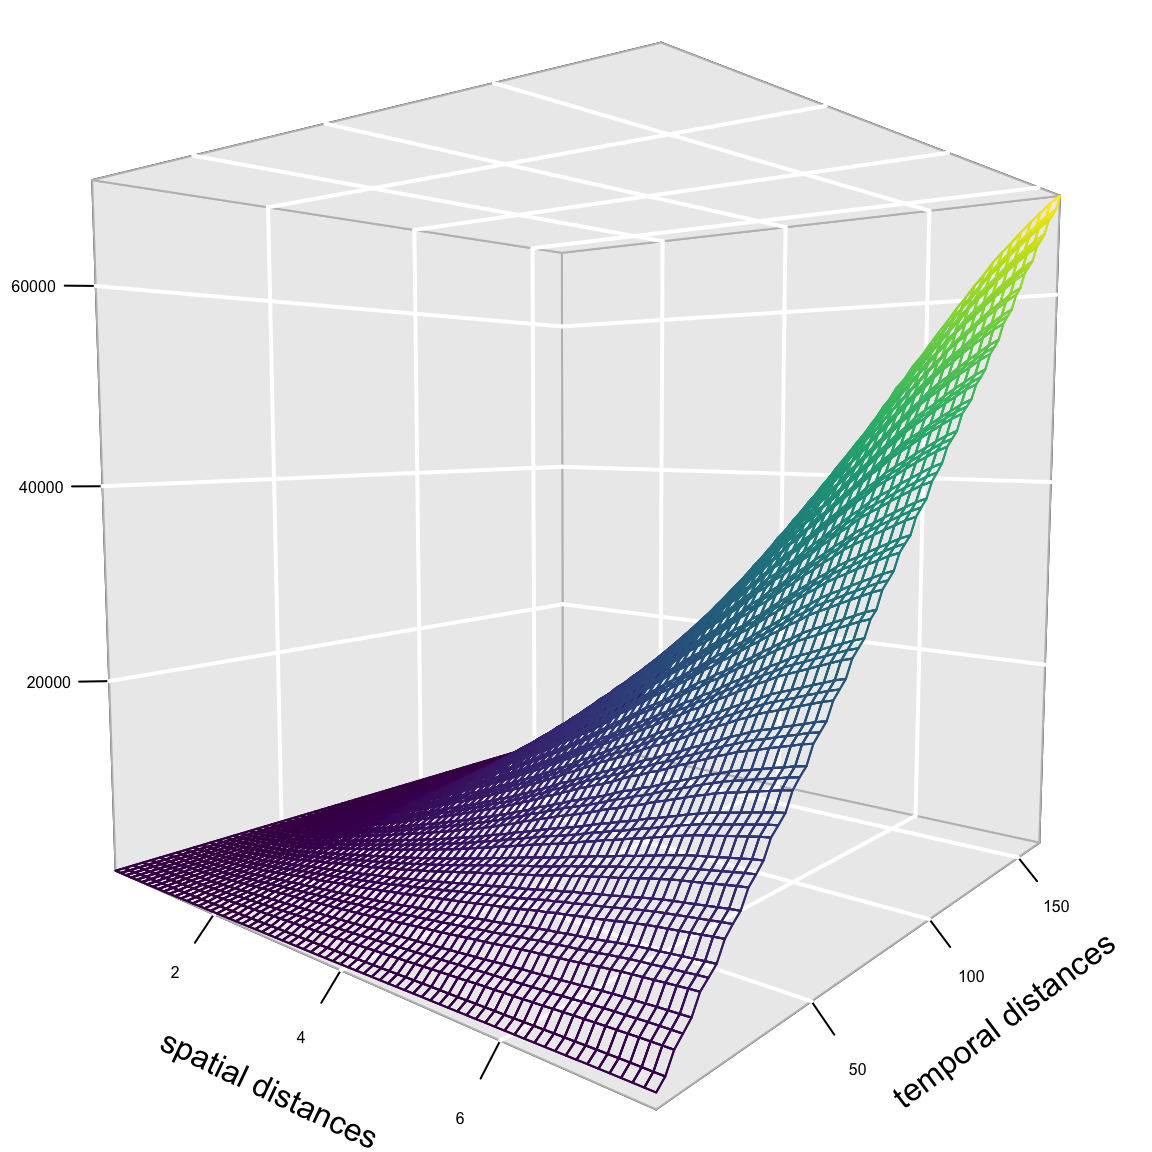
\includegraphics[width=0.65\linewidth]{stpointprocess_files/figure-latex/Kfunctions-1} 

}

\caption{Spatio-temporal pair correlation function estimate of non-specific gastrointestinal disease data.}\label{fig:Kfunctions}
\end{figure}

Figure \ref{fig:Kfunctions} shows the estimated \(K\)-function. Since the \(K\)-function is centred on its theoretical value \((2\pi r^2 t)\), we can easily interpret it; positive deviations suggest clustering, while negative deviations represent regularity or inhibition. In our case, we can see positive deviations that become larger as the spatial and temporal distances grow together. Therefore, as time passes and spatial distances become larger, the level of clustering also increases in our point pattern, at least in the range we have considered, that is, up to 7km in space and up to 5 months in time.

\hypertarget{discussion}{%
\section{Discussion}\label{discussion}}

Throughout this paper, we have shown how to analyse complex spatial and spatio-temporal point patterns through various techniques that aim to capture their first and second-order characteristics using several R packages. Specifically, we have toured very recent techniques such as variable bandwidths, relative risk inference, and composite hypotheses. The spatial methods presented are well-investigated and documented and can be easily applied using R. We have seen that some procedures, such as estimating \(p\)-values in composite hypotheses, require severe computational resources. The approximate computing time, including all the routines and set parameters suggested throughout the paper, is approximately six hours in a 3 GHz 6-Core Intel Core i5 iMac computer. This time depends on several factors, such as the number of simulations and the precision of desired outputs. It is mainly due to the number of points in the point pattern; the more data points, the more computational complexity, especially in the case of second-order descriptors, where pairwise calculations are required. Some R packages such as \pkg{foreach} can help accelerate the computations, even though these methods may quickly become unfeasible when the datasets have many points.

We have presented the most straightforward methods and the most widely known in the literature; we have done this, above all, because we intended to provide a solid and approachable learning resource. However, there are also alternative methods to deal with some of the descriptors we analyse in this document; for example, González and Moraga (2022a) presents a methodology to accurately and adaptively estimate the spatio-temporal intensity functions; this methodology can be applied using the \pkg{kernstadapt} package.

The analyses presented here can benefit future researchers who have initial questions about spatio-temporal point process data; these results can serve, for instance, as input for possible statistical models. We have not delved into statistical modelling and inference since many models exist in the spatio-temporal point processes literature. These statistical models can incorporate current knowledge of the phenomenon and many scientific considerations. Different models can be proposed and compared to decide which variables significantly influence the summary descriptors, making the results more informative (Adrian Baddeley, Rubak, and Turner 2015). For example, one of the most flexible families of models with the most methodological advantages is the family of log-Gaussian point processes. Log-Gaussian Cox processes are models for point patterns that intend to capture the environmental variability (Peter J. Diggle et al. 2013). They are spatio-temporal Poisson processes conditional on the realisation \(\lambda(\mathbf{u},v)\) of a stochastic intensity function \(\Lambda(\mathbf{u},v), (\mathbf{u},v)\in \mathbb{R}^2\times \mathbb{R}\). In the SOIRS case, a convenient representation of the intensity is
\[
    \log \left\{ \Lambda(\mathbf{u},v) \right\}= \lambda(\mathbf{u},v)S(\mathbf{u},v),
\]
where \(S(\mathbf{u},v)\) is a Gaussian stationary process with expectation \(1\) and covariance function \(\gamma(r,t)=\sigma^2 s(r,t)\), where \(\sigma^2\) is the variance of \(S(\mathbf{u}, v)\) and \(s(\cdot, \cdot)\) is a spatio-temporal correlation function, where \(r\) and \(t\) are spatial and temporal distances. Inference uses a discretised version of \(S(\mathbf{u},v)\), namely \(\mathcal{S}\), defined on a regular grid, where observations \(X\) are the cell counts, and the intensity of the process is assumed constant within each cell (B. Taylor and Diggle 2014). \(\mathcal{S}\) is a finite collection of Gaussian random variables, so its properties imply a multivariate Gaussian density. The covariance matrix elements are calculated by evaluating \(\gamma(r,t)\) at the centroids of the cells. Predictive inference about \(\mathcal{S}\) requires samples from the conditional distribution of the latent field given the observations, namely \([\mathcal{S}|X]\). For estimating the parameters of a space-time log-Gaussian Cox process, one can choose between computationally feasible methods, such as those based on moments or more demanding methods based on likelihood (Peter J. Diggle et al. 2013). Inference can be achieved for example, by using Markov chain Monte Carlo (MCMC) for which the \pkg{lgcp} package can be used, and by using integrated nested Laplace approximation (INLA) with the \pkg{inla} and \pkg{inlabru} packages.

To conclude, the methods presented here are primarily concerned with understanding the probability distribution that generate points observed in space or time. The study of such a distribution involves many routines, concepts and contexts that can help answer scientific questions and make decisions based on the data or inferences about them. The inclusion of technological advancements in R has led to improved efficiency and speed in calculations. Additionally, R offers a versatile and reliable environment for implementing statistical procedures and creating graphical visualisations. Also, modern developments in spatial statistics related to point patterns have been made possible thanks to the widespread availability of reproducible R scripts for analyses. In this paper, we have made extensive use of the ability to apply, extend and modify procedures in R to analyse spatial and spatio-temporal point patterns in the context of epidemiology. These approaches are also helpful for analysing point pattern data that arise in various fields such as climatology, ecology or seismology.

\hypertarget{references}{%
\section*{References}\label{references}}
\addcontentsline{toc}{section}{References}

\hypertarget{refs}{}
\begin{CSLReferences}{1}{0}
\leavevmode\vadjust pre{\hypertarget{ref-bachl2019inlabru}{}}%
Bachl, Fabian E, Finn Lindgren, David L Borchers, and Janine B Illian. 2019. {``{inlabru}: An {R} Package for {B}ayesian Spatial Modelling from Ecological Survey Data.''} \emph{Methods in Ecology and Evolution} 10 (6): 760--66.

\leavevmode\vadjust pre{\hypertarget{ref-baddeley2017twostage}{}}%
Baddeley, Adrian, Andrew Hardegen, Thomas Lawrence, Robin K. Milne, Gopalan Nair, and Suman Rakshit. 2017. {``On Two-Stage {M}onte {C}arlo Tests of Composite Hypotheses.''} \emph{Computational Statistics \& Data Analysis} 114: 75--87.

\leavevmode\vadjust pre{\hypertarget{ref-baddeley2015spatialR}{}}%
Baddeley, Adrian, Ege Rubak, and Rolf Turner. 2015. \emph{Spatial Point Patterns: Methodology and Applications with r}. Chapman \& Hall Interdisciplinary Statistics Series. CRC Press, Boca Raton, Florida.

\leavevmode\vadjust pre{\hypertarget{ref-baddeley2005}{}}%
Baddeley, A, and R Turner. 2005. {``{spatstat}: An {R} Package for Analyzing Spatial Point Patterns.''} \emph{Journal of Statistical Software} 12(6): 1--42.

\leavevmode\vadjust pre{\hypertarget{ref-besag1977}{}}%
Besag, Julian. 1977. {``Contribution to the Discussion of Dr {R}ipley's Paper.''} \emph{Journal of the Royal Statistical Society: Series B (Statistical Methodology)} 39: 193--95.

\leavevmode\vadjust pre{\hypertarget{ref-virgilio2013R}{}}%
Bivand, Roger S., Edzer Pebesma, and Virgilio Gómez-Rubio. 2013. \emph{Applied Spatial Data Analysis with {R}}. Second. Springer, New York.

\leavevmode\vadjust pre{\hypertarget{ref-choihall1999}{}}%
Choi, Edwin, and Peter Hall. 1999. {``Nonparametric Approach to Analysis of Space-Time Data on Earthquake Occurrences.''} \emph{Journal of Computational and Graphical Statistics} 8: 733--48.

\leavevmode\vadjust pre{\hypertarget{ref-daley2003}{}}%
Daley, D., and D. Vere-Jones. 2003. \emph{An Introduction to the Theory of Point Processes: Volume i: Elementary Theory and Methods}. Second. Springer-Verlag, New York.

\leavevmode\vadjust pre{\hypertarget{ref-davies2018relativerisksparr}{}}%
Davies, T. M., J. C. Marshall, and M. L. Hazelton. 2018. {``Tutorial on Kernel Estimation of Continuous Spatial and Spatiotemporal Relative Risk.''} \emph{Statistics in Medicine} 37 (7): 1191--221.

\leavevmode\vadjust pre{\hypertarget{ref-Davies2018kernel}{}}%
Davies, Tilman M., and Adrian Baddeley. 2018. {``Fast Computation of Spatially Adaptive Kernel Estimates.''} \emph{Statistics and Computing} 28 (4): 937--56.

\leavevmode\vadjust pre{\hypertarget{ref-diggle1985kernel}{}}%
Diggle, P. J. 1985. {``A Kernel Method for Smoothing Point Process Data.''} \emph{Journal of the Royal Statistical Society: Series C (Applied Statistics)} 34 (2): 138--47.

\leavevmode\vadjust pre{\hypertarget{ref-diggle2013book}{}}%
---------. 2013. \emph{Statistical Analysis of Spatial and Spatio-Temporal Point Patterns}. Third. Chapman \& Hall Monographs on Statistics \& Applied Probability. CRC Press, Boca Raton, Florida.

\leavevmode\vadjust pre{\hypertarget{ref-diggle2013paradigm}{}}%
Diggle, Peter J., Paula Moraga, Barry Rowlingson, and Benjamin Taylor. 2013. {``Spatial and Spatio-Temporal Log-{G}aussian {C}ox Processes: Extending the Geostatistical Paradigm.''} \emph{Statistical Science} 28: 542--63.

\leavevmode\vadjust pre{\hypertarget{ref-diggle2003aegis}{}}%
Diggle, P., L Knorr-Held, Rowlingson B, T Su, Pand Hawtin, and T Bryant. 2003. {``On-Line Monitoring of Public Health Surveillance Data.''} In \emph{Monitoring the Health of Populations: Statistical Principlesand Methods for Public Health Surveillance}, edited by Brookmeyer R. and Stroup D. F., 233--66. Oxford University Press.

\leavevmode\vadjust pre{\hypertarget{ref-gabriel2013raey}{}}%
Gabriel, Edith. 2014. {``Estimating Second-Order Characteristics of Inhomogeneous Spatio-Temporal Point Processes.''} \emph{Methodology and Computing in Applied Probability} 16: 411--31.

\leavevmode\vadjust pre{\hypertarget{ref-diggle2009}{}}%
Gabriel, Edith, and Peter J. Diggle. 2009. {``Second-Order Analysis of Inhomogeneous Spatio-Temporal Point Process Data.''} \emph{Statistica Neerlandica} 63 (1): 43--51.

\leavevmode\vadjust pre{\hypertarget{ref-gabriel2013stpp}{}}%
Gabriel, Edith, Barry Rowlingson, and Peter J. Diggle. 2013. {``{stpp}: An {\texttt{R}} Package for Plotting, Simulating and Analyzing Spatio-Temporal Point Patterns.''} \emph{Journal of Statistical Software} 53(2) (2): 1--29.

\leavevmode\vadjust pre{\hypertarget{ref-viridispackage}{}}%
Garnier, Simon, Simon, Noam Ross, Bob Rudis, Marco Sciaini, Antonio Pedro, and Cedric Scherer. 2023. \emph{\texttt{viridis(Lite)} - Colorblind-Friendly Color Maps for \texttt{R}}. \url{https://doi.org/10.5281/zenodo.4679424}.

\leavevmode\vadjust pre{\hypertarget{ref-ghorbani2021separability}{}}%
Ghorbani, Mohammad, Nafiseh Vafaei, Jiří Dvořák, and Mari Myllymäki. 2021. {``Testing the First-Order Separability Hypothesis for Spatio-Temporal Point Patterns.''} \emph{Computational Statistics \& Data Analysis} 161: 107245.

\leavevmode\vadjust pre{\hypertarget{ref-gonzalez2019tornadoes}{}}%
González, Jonatan A., Ute Hahn, and Jorge Mateu. 2019. {``Analysis of Tornado Reports Through Replicated Spatiotemporal Point Patterns.''} \emph{Journal of the Royal Statistical Society: Series C (Applied Statistics)} 69 (1): 3--23.

\leavevmode\vadjust pre{\hypertarget{ref-adaptiveGonzalez2022arxiv}{}}%
González, Jonatan A., and Paula Moraga. 2022a. {``An Adaptive Kernel Estimator for the Intensity Function of Spatio-Temporal Point Processes.''} arXiv. \url{https://doi.org/10.48550/ARXIV.2208.12026}.

\leavevmode\vadjust pre{\hypertarget{ref-kernstadaptpackage}{}}%
---------. 2022b. {``\texttt{kernstadapt}: Spatio-Temporal Adaptive Kernel Estimators for Intensities.''} https://doi.org/\url{https://CRAN.R-project.org/package=kernstadapt}.

\leavevmode\vadjust pre{\hypertarget{ref-gonzalezetal2016}{}}%
González, Jonatan A., Francisco J. Rodríguez-Cortés, Ottmar Cronie, and Jorge Mateu. 2016. {``Spatio-Temporal Point Process Statistics: A Review.''} \emph{Spatial Statistics} 18: 505--44.

\leavevmode\vadjust pre{\hypertarget{ref-harte2010PtProcess}{}}%
Harte, David. 2010. {``{PtProcess}: An {R} Package for Modelling Marked Point Processes Indexed by Time.''} \emph{Journal of Statistical Software} 35 (8): 1--32.

\leavevmode\vadjust pre{\hypertarget{ref-hazelton2009inferenceRelativeRisk}{}}%
Hazelton, Martin L., and Tilman M. Davies. 2009. {``Inference Based on Kernel Estimates of the Relative Risk Function in Geographical Epidemiology.''} \emph{Biometrical Journal} 51 (1): 98--109.

\leavevmode\vadjust pre{\hypertarget{ref-illian2008}{}}%
Illian, J., P. A. Penttinen, H. Stoyan, and D. Stoyan. 2008. \emph{Statistical Analysis and Modelling of Spatial Point Patterns}. Statistics in Practice. Wiley.

\leavevmode\vadjust pre{\hypertarget{ref-jalilian2018fastpcfbandwidth}{}}%
Jalilian, Abdollah, and Rasmus Waagepetersen. 2018. {``Fast Bandwidth Selection for Estimation of the Pair Correlation Function.''} \emph{Journal of Statistical Computation and Simulation} 88 (10): 2001--11.

\leavevmode\vadjust pre{\hypertarget{ref-kelsalDiggle1995risk}{}}%
Kelsall, Julia E., and Peter J. Diggle. 1995. {``Kernel Estimation of Relative Risk.''} \emph{Bernoulli} 1 (1/2): 3--16.

\leavevmode\vadjust pre{\hypertarget{ref-doparallelpackage}{}}%
Microsoft, and Steve Weston. 2022a. \emph{\texttt{doParallel}: Foreach Parallel Adaptor for the 'Parallel' Package}. \url{https://CRAN.R-project.org/package=doParallel}.

\leavevmode\vadjust pre{\hypertarget{ref-foreachpackage}{}}%
---------. 2022b. \emph{\texttt{foreach}: Provides Foreach Looping Construct}. \url{https://CRAN.R-project.org/package=foreach}.

\leavevmode\vadjust pre{\hypertarget{ref-Moller2012}{}}%
Møller, M, J. And Ghorbani. 2012. {``Aspects of Second-Order Analysis of Structured Inhomogeneous Spatio-Temporal Point Processes.''} \emph{Statistica Neerlandica} 66: 472--91.

\leavevmode\vadjust pre{\hypertarget{ref-moraga2019geospatial}{}}%
Moraga, Paula. 2019. \emph{Geospatial Health Data: Modeling and Visualization with {R-INLA} and Shiny}. Biostatistics Series. Chapman \& Hall/CRC, Boca Raton, Florida.

\leavevmode\vadjust pre{\hypertarget{ref-moraga21}{}}%
---------. 2021. {``Species Distribution Modeling Using Spatial Point Processes: A Case Study of Sloth Occurrence in {C}osta {R}ica.''} \emph{The {R} Journal} 12 (2): 293--310.

\leavevmode\vadjust pre{\hypertarget{ref-moraga2011lisavsscan}{}}%
Moraga, Paula, and Francisco Montes. 2011. {``Detection of Spatial Disease Clusters with LISA Functions.''} \emph{Statistics in Medicine} 30 (10): 1057--71.

\leavevmode\vadjust pre{\hypertarget{ref-get2020package}{}}%
Myllymäki, Mari, and Tomáš Mrkvička. 2020. {``{GET}: Global Envelopes in {R}.''} \emph{arXiv:1911.06583 {[}Stat.ME{]}}. \url{https://arxiv.org/abs/1911.06583}.

\leavevmode\vadjust pre{\hypertarget{ref-tomasute2017}{}}%
Myllymäki, Mari, Tomáš Mrkvička, Pavel Grabarnik, Henri Seijo, and Ute Hahn. 2017. {``Global Envelope Tests for Spatial Processes.''} \emph{Journal of the Royal Statistical Society: Series B (Statistical Methodology)} 79 (2): 381--404.

\leavevmode\vadjust pre{\hypertarget{ref-pebesma2005SP}{}}%
Pebesma, E. J., and Roger S. B. 2005. {``Classes and Methods for Spatial Data in {R}.''} \emph{R News} 5 (2): 9--13.

\leavevmode\vadjust pre{\hypertarget{ref-pebesma2018SF}{}}%
Pebesma, Edzer. 2018. {``Simple Features for {R}: Standardized Support for Spatial Vector Data.''} \emph{The {R} Journal} 10 (1): 439--46.

\leavevmode\vadjust pre{\hypertarget{ref-rcoreteam}{}}%
R Core Team. 2023. \emph{\texttt{R}: A Language and Environment for Statistical Computing}. Vienna, Austria: {R} Foundation for Statistical Computing. \url{https://www.R-project.org}.

\leavevmode\vadjust pre{\hypertarget{ref-ripley1977}{}}%
Ripley, B D. 1977. {``Modelling Spatial Patterns (with Discussion).''} \emph{Journal of the Royal Statistical Society: Series B (Statistical Methodology)} 39 (2): 172--212.

\leavevmode\vadjust pre{\hypertarget{ref-rodrigues:diggle:12}{}}%
Rodrigues, Alexandre, and Peter J. Diggle. 2012. {``Bayesian Estimation and Prediction for Inhomogeneous Spatiotemporal Log-{G}aussian {C}ox Processes Using Low-Rank Models, with Application to Criminal Surveillance.''} \emph{Journal of the American Statistical Association} 107 (497): 93--101.

\leavevmode\vadjust pre{\hypertarget{ref-rowlingson1993SPLANCS}{}}%
Rowlingson, B. S, and P. J Diggle. 1993. {``{splancs}: Spatial Point Pattern Analysis Code in {S-PLUS}.''} \emph{Computers \& Geosciences} 19 (5): 627--55.

\leavevmode\vadjust pre{\hypertarget{ref-rue2009royal}{}}%
Rue, Håvard, Sara Martino, and Nicolas Chopin. 2009. {``Approximate Bayesian Inference for Latent {G}aussian Models by Using Integrated Nested {L}aplace Approximations.''} \emph{Journal of the Royal Statistical Society: Series B (Statistical Methodology)} 71 (2): 319--92.

\leavevmode\vadjust pre{\hypertarget{ref-scott2015multivariate}{}}%
Scott, David W. 2015. \emph{Multivariate Density Estimation: Theory, Practice, and Visualization}. Second. Wiley Series in Probability and Statistics. John Wiley \& Sons.

\leavevmode\vadjust pre{\hypertarget{ref-sheather1991bandwidth}{}}%
Sheather, S. J., and M. C. Jones. 1991. {``A Reliable Data-Based Bandwidth Selection Method for Kernel Density Estimation.''} \emph{Journal of the Royal Statistical Society: Series B (Statistical Methodology)} 53 (3): 683--90.

\leavevmode\vadjust pre{\hypertarget{ref-silverman1986density}{}}%
Silverman, Bernard W. 1986. \emph{Density Estimation for Statistics and Data Analysis}. Chapman \& Hall Monographs on Statistics \& Applied Probability. CRC press, Boca Raton, Florida.

\leavevmode\vadjust pre{\hypertarget{ref-taylor2013lgcp}{}}%
Taylor, Benjamin M, Tilman M Davies, Barry S Rowlingson, and Peter J Diggle. 2013. {``Lgcp: An {R} Package for Inference with Spatial and Spatio-Temporal Log-{G}aussian {C}ox Processes.''} \emph{Journal of Statistical Software} 52: 1--40.

\leavevmode\vadjust pre{\hypertarget{ref-taylordiggle2014}{}}%
Taylor, Benjamin, and Peter Diggle. 2014. {``{INLA} or {MCMC}? A Tutorial and Comparative Evaluation for Spatial Prediction in Log-{G}aussian {C}ox Processes.''} \emph{Journal of Statistical Computation and Simulation} 84 (10): 2266--84.

\leavevmode\vadjust pre{\hypertarget{ref-turner2009}{}}%
Turner, Rolf. 2009. {``Point Patterns of Forest Fire Locations.''} \emph{Environmental and Ecological Statistics} 16 (2): 197--223.

\leavevmode\vadjust pre{\hypertarget{ref-ripley2002}{}}%
Venables, W. N., and B. D. Ripley. 2002. \emph{Modern Applied Statistics with s}. Fourth. Statistics and Computing. Springer-Verlag, New York.

\leavevmode\vadjust pre{\hypertarget{ref-wassle1981morphology}{}}%
Wässle, H, Brian Blundell Boycott, and R-B Illing. 1981. {``Morphology and Mosaic of on-and Off-Beta Cells in the Cat Retina and Some Functional Considerations.''} \emph{Proceedings of the Royal Society of London. Series B. Biological Sciences} 212 (1187): 177--95.

\leavevmode\vadjust pre{\hypertarget{ref-ggplot2package}{}}%
Wickham, Hadley. 2016. \emph{\texttt{ggplot2}: Elegant Graphics for Data Analysis}. Second. Springer-Verlag, New York.

\leavevmode\vadjust pre{\hypertarget{ref-wong2020}{}}%
Wong, Ka Yiu, and Dietrich Stoyan. 2021. {``Poles of Pair Correlation Functions: When They Are Real?''} \emph{Annals of the Institute of Statistical Mathematics} 73: 425--40.

\end{CSLReferences}

\bibliography{bibliography.bib}

\address{%
Jonatan A. González\\
King Abdullah University of Science and Technology (KAUST)\\%
Computer, Electrical and Mathematical Sciences and Engineering Division\\ Thuwal, 23955-6900, Saudi Arabia\\
%
%
\textit{ORCiD: \href{https://orcid.org/0000-0002-2296-5271}{0000-0002-2296-5271}}\\%
\href{mailto:jonathan.gonzalez@kaust.edu.sa}{\nolinkurl{jonathan.gonzalez@kaust.edu.sa}}%
}

\address{%
Paula Moraga\\
King Abdullah University of Science and Technology (KAUST)\\%
Computer, Electrical and Mathematical Sciences and Engineering Division\\ Thuwal, 23955-6900, Saudi Arabia\\
%
\url{http://www.paulamoraga.com}\\%
\textit{ORCiD: \href{https://orcid.org/0000-0001-5266-0201}{0000-0001-5266-0201}}\\%
\href{mailto:paula.moraga@kaust.edu.sa}{\nolinkurl{paula.moraga@kaust.edu.sa}}%
}
